\documentclass[a4paper]{article}
\usepackage[normalem]{ulem}
\usepackage{graphicx}
\usepackage[font=small,labelfont=bf]{caption}

% impostazioni generali
%Tutti gli usepackage vanno qui
\usepackage[table]{xcolor}
\usepackage{geometry}
\usepackage[italian]{babel}
\usepackage[utf8]{inputenc}
\usepackage{tabularx}
\usepackage{longtable}
\usepackage{hyperref}
\usepackage{enumitem}
\usepackage{array} 
\usepackage{booktabs}
\newcolumntype{M}[1]{>{\centering\arraybackslash}m{#1}}
\usepackage[toc]{appendix}
\usepackage{caption}

\hypersetup{
	colorlinks=true,
	linkcolor=blue,
	filecolor=magenta,
	urlcolor=blue,
}
% Numerazione figure
\let\counterwithout\relax
\let\counterwithin\relax
\usepackage{chngcntr}

% distanziare elenco delle figure e delle tabelle
\usepackage{tocbasic}
\DeclareTOCStyleEntry[numwidth=3.5em]{tocline}{figure}% for figure entries
\DeclareTOCStyleEntry[numwidth=3.5em]{tocline}{table}% for table entries


%\counterwithout{table}{section}
%\counterwithout{figure}{section}
\captionsetup[table]{font=small,skip=5pt} 

\usepackage[bottom]{footmisc}
\usepackage{fancyhdr}
\setcounter{secnumdepth}{4}
\usepackage{amsmath, amssymb}
\usepackage{array}
\usepackage{graphicx}

\usepackage{ifthen}

\usepackage{float}
\restylefloat{table}

\usepackage{layouts}
\usepackage{url}
\usepackage{comment}
\usepackage{eurosym}

\usepackage{lastpage}
\usepackage{layouts}
\usepackage{eurosym}

\geometry{a4paper,top=3cm,bottom=4cm,left=2.5cm,right=2.5cm}

%Comandi di impaginazione uguale per tutti i documenti
\pagestyle{fancy}
\lhead{
\includegraphics[scale=0.25]{template/images/logo-inline.png}}


%\rfoot{\thepage}
\cfoot{Pagina \thepage\ di \pageref{LastPage}}
\setlength{\headheight}{35pt}
\setcounter{tocdepth}{5}
\setcounter{secnumdepth}{5}
\renewcommand{\footrulewidth}{0.4pt}

% multirow per tabelle
\usepackage{multirow}

% Permette tabelle su più pagine
%\usepackage{longtable}


%COMANDI TABELLE
\newcommand{\rowcolorhead}{\rowcolor[HTML]{731733}}
\newcommand{\captionline}{\rowcolor[HTML]{FFFFFF}} %comando per le caption delle tabelle
\newcommand{\cellcolorhead}{\cellcolor[HTML]{007c95}}
\newcommand{\hlinetable}{\arrayrulecolor[HTML]{007c95}\hline}

%intestazione
% check for missing commands
\newcommand{\headertitle}[1]{\textbf{\color{white}#1}} %titolo colonna
\definecolor{pari}{HTML}{dcbac2}
\definecolor{dispari}{HTML}{f5f5f5}

% comandi \textit{Glossario}
\newcommand{\glo}{$_{G}$}
\newcommand{\glosp}{$_{G}$ }


%label custom
\makeatletter
\newcommand{\uclabel}[2]{%
	\protected@write \@auxout {}{\string \newlabel {#1}{{#2}{\thepage}{#2}{#1}{}} }%
	\hypertarget{#1}{#2}
}
\makeatother

%riportare pezzi di codice
\definecolor{codegray}{gray}{0.9}
\newcommand{\code}[1]{\colorbox{codegray}{\texttt{#1}}}

% dati relativi alla prima pagina
\makeindex
\begin{document}
\counterwithin{table}{section}

% Prima pagina
\thispagestyle{empty}
\renewcommand{\arraystretch}{1.3}


\begin{titlepage}
	\begin{center}
		
	
\includegraphics[scale = 0.7]{template/images/logo-circle.png}
	\\[1cm]
	\href{mailto:6bitbusters@gmail.com}		      	
	{\large{\textit{6bitbusters@gmail.com} } }\\[1cm]
	
	\Huge \textbf{Analisi dei requisiti} \\[1cm]

	% Informazioni sul documento
	\large \textbf{Informazioni sul documento} \\
	\rule{0.6\textwidth}{0.4pt}
	\\[0.5cm]
	\begin{tabular}{r|l}
		\textbf{Versione} & 0.8.0\\
		\textbf{Stato} & in redazione\\
		\textbf{Uso} & esterno\\                         
		\textbf{Approvazione} & -\\                      
		\textbf{Redazione} & Pincin Matteo\\ & Diviesti Filippo\\ & Soranzo Andrea \\ & Djossa Edgar \\
		\textbf{Verifica} & Bergamin Elia\\ & Soranzo Andrea \\ & Chilese Elena \\  & Djossa Edgar \\                     
		\textbf{Distribuzione} & \parbox[t]{5cm}{ \textit{Six Bit Busters} \\ Prof. Vardanega Tullio 
	 \\ Prof. Cardin Riccardo}
	\end{tabular}	
	\\[1.2cm]

 % Descrizione
	\large \textbf{Descrizione} \\ Documento di rendicontazione dell'\textit{Analisi dei requisiti}
	
	
	\end{center}
\end{titlepage}


% Diario delle modifiche

\section*{Registro delle modifiche}

\newcommand{\changelogTable}[1]{

\renewcommand{\arraystretch}{1.5}
\rowcolors{2}{pari}{dispari}
\begin{longtable}{ %0.87
		>{\centering}M{0.10\textwidth} 
		>{\centering}M{0.11\textwidth}
		>{\centering}M{0.19\textwidth}
		>{\centering}M{0.28\textwidth} 
		>{\centering\arraybackslash}M{0.19\textwidth} 
		 }
	\rowcolorhead
	\headertitle{Versione} &
	\centering \headertitle{Data} &	
	\headertitle{Autore} &
	\headertitle{Descrizione} & 
	\headertitle{Verificatore} 
	\endfirsthead	
	\endhead
	
	#1

\end{longtable}
\vspace{-2em}

}
% Insert changelog values here
\changelogTable{
  2.0.1 & 19-03-2025 & Soranzo Andrea & Rimossi numeri di sezione & - \tabularnewline
  2.0.0 & 02-03-2025 & Soranzo Andrea & Approvazione documento & - \tabularnewline
	1.1.0 & 02-03-2025 & Bergamin Elia & Integrazione vocaboli & Djossa Edgar \tabularnewline
	1.0.0 & 31-01-2025 & Soranzo Andrea & Approvazione documento & - \tabularnewline
	0.7.0 & 30-01-2025 & Chilese Elena & Revisione documento & Bergamin Elia \tabularnewline
	0.6.0 & 28-01-2025 & Bergamin Elia & Integrazione vocaboli & Pincin Matteo \tabularnewline
	0.5.0 & 10-01-2025 & Diviesti Filippo & Integrazione vocaboli & Soranzo Andrea\tabularnewline
    0.4.0 & 16-12-2024 & Djossa Edgar & Integrazione vocaboli & Chilese Elena \tabularnewline   
	0.3.0 & 10-12-2024 & Bergamin Elia & Aggiunta Introduzione, integrazione vocaboli e morfologia & Djossa Edgar \tabularnewline
	0.2.0 & 25-11-2024 & Bergamin Elia & Integrazione vocaboli & Soranzo Andrea \tabularnewline
	0.1.0 & 19-11-2024 & Diviesti Filippo & Inserimento vocaboli per \textit{Norme di progetto} e \textit{Piano di progetto} & Pincin Matteo \\
}

\pagebreak

% Indice
{
    \hypersetup{linkcolor=black}
    \tableofcontents
}
\pagebreak

% Tabelle 
{
    \listoftables
}
\pagebreak

% Figure
{
    \listoffigures
}

% Contenuto
%

\pagebreak

\section{Analisi dei rischi}
In questa sezione sono riassunti i rischi a cui il gruppo si espone a seguito dell'aggiudicazione del capitolato 3Dataviz.
\pagebreak

\section{Modello di sviluppo}
\subsection{Modello agile}
Il gruppo \textit{Six Bit Busters} ha deciso di adottare un approccio ispirato
ai modelli agili, cercando di avvicinarsi il più possibile alle metodologie
tipiche del framework \textbf{Scrum}. Questa scelta è motivata dalle seguenti
considerazioni:
\begin{itemize}
    \item Scrum promuove la \textbf{collaborazione} continua tra i membri del team e gli
          stakeholder;
    \item Grazie agli sprint brevi, Scrum consente di \textbf{adattarsi} rapidamente a
          nuove esigenze o priorità;
    \item Gli sprint brevi consentono di individuare e \textbf{risolvere i problemi} più
          velocemente;
    \item Ad ogni sprint, il team si concentra su un \textbf{numero limitato di
              attività}, aumentando l'efficienza;
    \item I membri del team decidono come svolgere il lavoro durante gli sprint,
          aumentando il senso di \textbf{responsabilità};
    \item La natura iterativa di Scrum aiuta a suddividere grandi obiettivi in attività
          più \textbf{piccole e realizzabili}.
\end{itemize}

\subsection{Ruoli Scrum}
Scrum prevede tre ruoli (anche detti "responsabilità") che garantiscono che
ogni aspetto del lavoro condiviso sia gestito in modo efficace:
\begin{itemize}
    \item \textbf{Sviluppatori}: lavorano insieme per creare qualsiasi
          aspetto del prodotto. Le persone con qualsiasi competenza necessaria
          per creare il prodotto assumono la responsabilità di sviluppatore. Nel
          progetto didattico, tutti i membri del team ricoprono tale ruolo;
    \item \textbf{Product owner}: sviluppa e comunica l'obiettivo del prodotto
          ed è responsabile del product back-log. % trattino per andare a capo bene% 
          Conosce e comprende il dominio e il
          mercato del prodotto e vuole fornire agli utenti ciò di cui hanno bisogno.
          Nel progetto didattico, il product owner è il proponente;
    \item \textbf{Scrum master}: guida e dirige il team nell'adozione e
          nella pratica di Scrum. In particolare cerca di massimizzare l'utilità
          degli eventi e degli artefatti. Nel progetto didattico, lo Scrum master è
          il membro del team con il ruolo di responsabile.
\end{itemize}

\subsection{Eventi Scrum}
Gli eventi Scrum sono preziose opportunità per ispezionare e adattare il
prodotto o il modo in cui il team lavora insieme.
\begin{itemize}
    \item \textbf{Sprint}: è un breve periodo di tempo in cui il team collabora per
          completare una determinata quantità di lavoro. Lo sprint contiene tutti gli altri eventi.
          Per il gruppo \textit{Six Bit Busters} ogni sprint dura due settimane;
    \item \textbf{Sprint planning}: stabilisce l'obiettivo dello sprint.
          Gli sviluppatori prevedono quali lavori ritengono di poter realizzare durante
          lo sprint per raggiungere l'obiettivo e come verrà completato il lavoro scelto.
          In base all'obiettivo viene creato un piano iniziale;
    \item \textbf{Daily scrum}: incontro giornaliero a cui partecipano tutti i membri del team,
          in cui ciascuno risponde alle seguenti domande:
          \begin{itemize}
              \item Cosa hai fatto ieri?
              \item Cosa farai oggi?
              \item C'è qualcosa che ti impedisce di farlo?
          \end{itemize}
          Ogni giorno lavorativo, al mattino, si svolge il daily scrum su un gruppo Telegram dedicato;
    \item \textbf{Sprint review}: il team esamina l'esito dello sprint con il
          product owner, che fornisce feedback su ciò che il team ha realizzato
          e sulla futura direzione dello sviluppo del prodotto. Il product backlog
          viene adattato in base a queste conversazioni;
    \item \textbf{Sprint retrospective}: è l'opportunità per il team di analizzare le
          proprie interazioni, collaborazioni, processi, strumenti e qualsiasi altro fattore
          ritenuto rilevante per la propria capacità di migliorare continuamente.
\end{itemize}

\subsection{Artefatti Scrum}
\begin{itemize}
    \item \textbf{Product backlog}: elenco ordinato o classificato di tutto ciò che potrebbe
          essere necessario per migliorare il prodotto, insieme all'obiettivo del prodotto;
    \item \textbf{Sprint backlog}: è composto dall'obiettivo dello sprint e dal set di
          elementi del product backlog che il product owner e gli sviluppatori hanno previsto
          di poter completare durante lo sprint corrente;
    \item \textbf{Incremento}: elemento del backlog completato in modo da fornire valore
          ed essere utilizzabile.
\end{itemize}
\subsection{Principi fondamentali}
\begin{itemize}
    \item \textbf{Trasparenza}: per prendere decisioni efficaci è necessario
          che il processo e i progressi del prodotto siano trasparenti,
          per garantire che tutti capiscano cosa stanno vedendo;
    \item \textbf{Ispezione}: le ispezioni regolari dei lavori in corso sono
          essenziali per mantenere il processo previsto e ottenere il risultato desiderato.
    \item \textbf{Adattamento}: consiste nell'esecuzione di tempestivi aggiustamenti
          al processo o al prodotto ogni volta che si verificano delle deviazioni. Ciò si
          realizza adattando il product backlog, il prodotto e i piani futuri a ogni sprint.\\\\
\end{itemize}

\begin{figure}[h!]
    \centering
    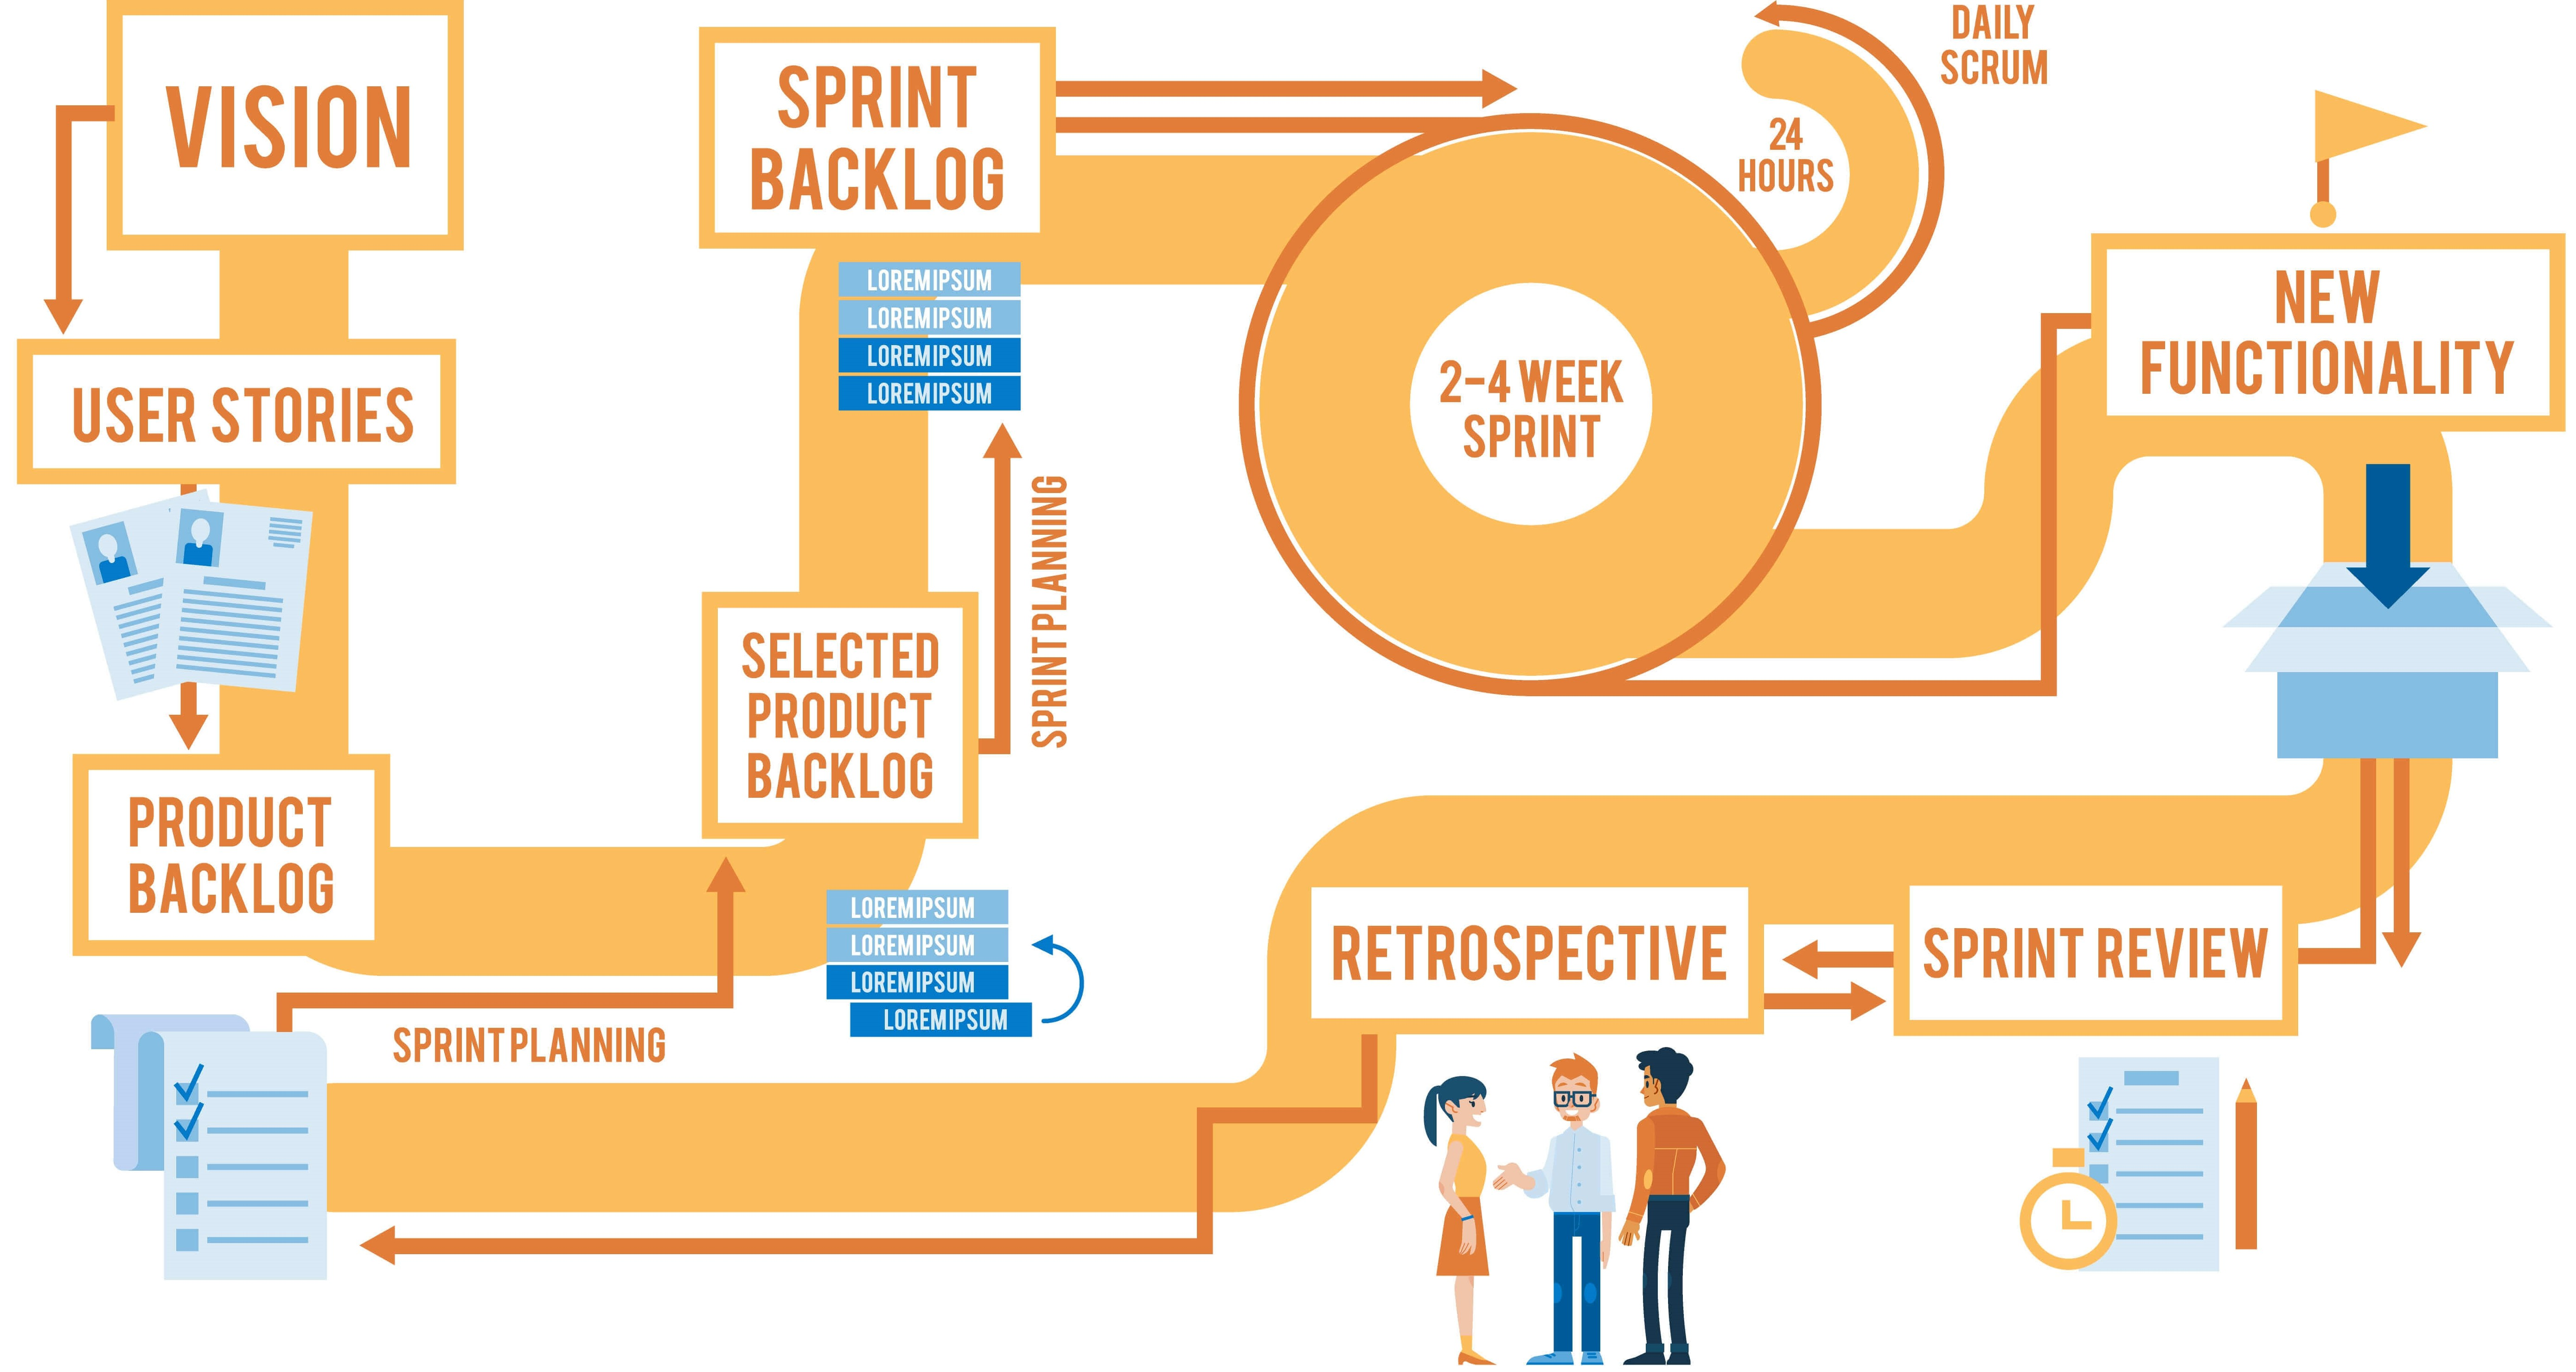
\includegraphics[scale = 0.08]{template/images/scrum.jpg}
    \caption{Il framework Scrum}
    \label{fig:2.1} % Etichetta per il riferimento
\end{figure}
\pagebreak

\section{Pianificazione}
Lo sviluppo del progetto è suddiviso nelle seguenti fasi:
    \begin{itemize}
        \item  RTB
        \item PB
    \end{itemize}
    \subsection{RTB}
    Nel periodo dal 04/11/2024 al 17/01/2025 verranno prodotti i seguenti documenti:
        \begin{itemize}
            \item "Norme di progetto"
            \item "Piano di progetto"
            \item "Analisi dei requisiti"
            \item "Piano di qualifica"
            \item "Glossario"
        \end{itemize}
    Inoltre verrà realizzato il Proof of Concept, per valutare la fattibilità tecnologica del progetto.
        \subsubsection{Sprint 1 (dal 11/11/2024 al 22/11/2024)}
        In questo periodo verrà definito il way of working, documentato nelle
        \textit{"Norme di progetto"}. Per quanto riguarda la gestione di progetto, verranno 
        pianificate le attività, stilato un preventivo e analizzati i rischi che potrebbero
        incidere sullo svolgimento del progetto. Infine si comincerà a redigere il 
        \textit{"Glossario"}, fondamentale per garantire una chiara comprensione e comunicazione all'
        interno del team e con il proponente.
        \\
        \begin{figure}[h!]
            \centering
            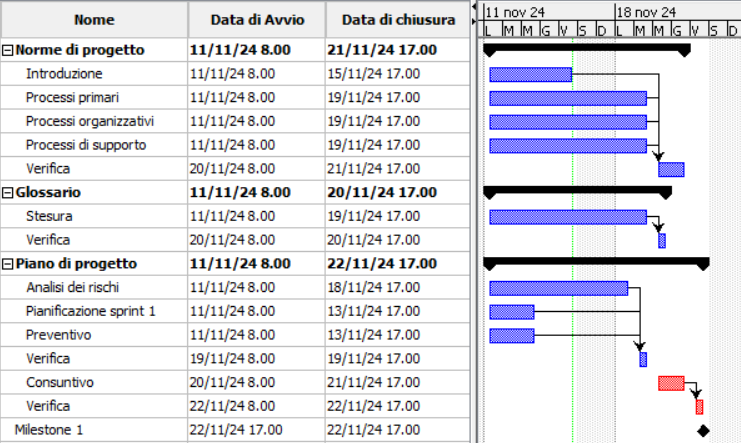
\includegraphics[scale = 0.85]{template/images/gantt1.png}
            \caption{Diagramma di Gantt sprint 1}
            \label{fig:3.1} % Etichetta per il riferimento
        \end{figure}

        \subsubsection{Sprint 2 (dal 25/11/2024 al 06/12/2024)}
     Durante questo secondo sprint, ci dedicheremo alla raccolta e all'analisi dei requisiti, identificando i casi d'uso. Questi saranno documentati nel file \textit{"Analisi dei requisiti"} per garantire una visione chiara degli obiettivi del progetto. Continueremo inoltre l'espansione del \textit{"glossario"}, già avviato durante lo sprint 1.  Procederemo con l'aggiornamento delle \textit{"Norme di Progetto"} tramite modifiche e miglioramenti per assicurare una gestione ottimale delle attività e delle risorse. infine, con priorità minore, inizieremo la stesura del \textit{"Piano di Qualifica"}, necessario per definire le metriche e le modalità di 
     verifica della qualità del prodotto.

        
        \begin{figure}[h!]
            \centering
            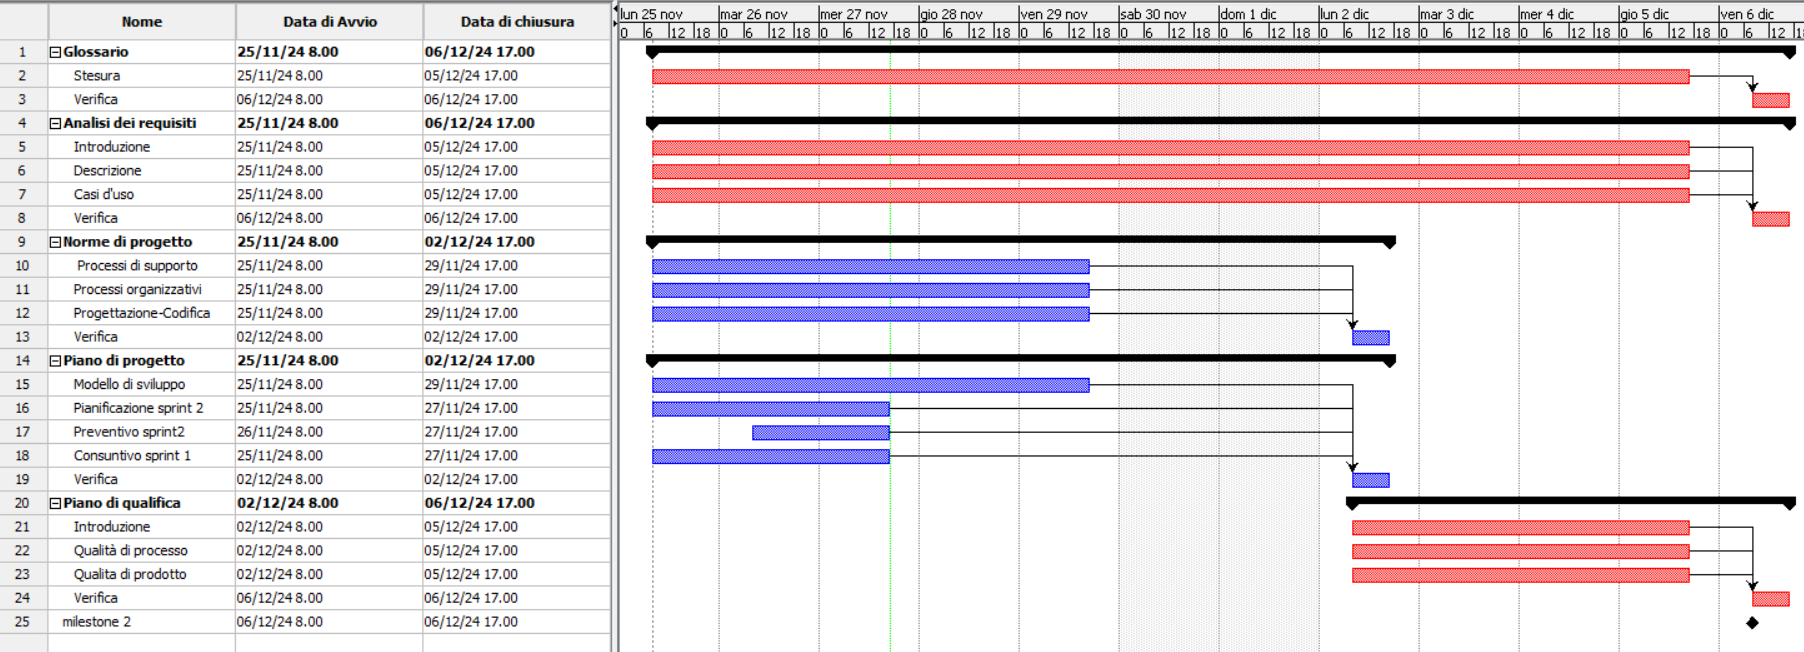
\includegraphics[scale = 0.3]{template/images/gantt2.png}
            \caption{Diagramma di Gantt sprint 2}
            \label{fig:3.1} % Etichetta per il riferimento
        \end{figure}
 

\pagebreak

\section{Preventivo}
In questa sezione viene pianificata nel dettaglio la suddivisione dei ruoli con
le corrispondenti ore di lavoro per ogni componente del gruppo e viene fornito
un preventivo, sia relativamente all'intera durata del progetto, sia
relativamente ad ogni periodo di lavoro.

\subsection{Ore totali}
Il team ha deciso di suddividere le ore individuali in modo equivalente,
assegnando un totale di 92 ore a ciascun membro. Di seguito si riporta la
distribuzione delle ore per ruolo e il calcolo dei costi totali.


\newcommand{\roleTable}[1]{

	\renewcommand{\arraystretch}{1.5}
	\rowcolors{2}{pari}{dispari}
	\begin{longtable}{ %0.87
		>{\centering}M{0.20\textwidth}
		>{\centering}M{0.10\textwidth}
		>{\centering}M{0.10\textwidth}
		>{\centering}M{0.10\textwidth}
		>{\centering\arraybackslash}M{0.15\textwidth}
		}
		\rowcolorhead
		\headertitle{Ruolo}           &
		\centering
		\headertitle{Ore ind.}        &
		\headertitle{Ore tot.}        &
		\headertitle{Costo (\euro/h)} &
		\headertitle{Costo Totale (\euro)}
		\endfirsthead
		\endhead

		#1

	\end{longtable}
	\vspace{1em}

}

    \roleTable{
    Responsabile& 9 & 54 & 30 &  1620\tabularnewline
    Amministratore& 7 & 42 & 20 &  840\tabularnewline
    Analista& 16 & 96 & 25 &  2400\tabularnewline
	Progettista& 20 & 120 & 25 &  3000\tabularnewline
	Programmatore & 22 & 132 & 15 &  1980 \\
    	Verificatore& 18 & 108 & 15 &  1620\tabularnewline
     \midrule[\heavyrulewidth] 
     \textbf{TOTALE}& 92 & 552 & - &  11460\tabularnewline

     \rowcolor{white}\caption{Distribuzione delle ore e costi totali}
    }





\subsection{Costo Totale}
Il costo finale calcolato in base alle tariffe orarie dei ruoli e alle ore
preventivate risulta di: \textbf{\euro 11460}.
\pagebreak
\subsection{RTB}
\subsubsection{Sprint 1}
Per il primo sprint, i ruoli necessari per raggiungere gli obiettivi
pianificati sono:
\begin{itemize}
    \item Responsabile;
    \item Amministratore;
    \item Verificatore;
    \item Analista.
\end{itemize}

Di seguito una tabella dettagliata con la distribuzione dei ruoli e delle ore previsti per ciascun membro.


\newcommand{\memberTable}[1]{

\renewcommand{\arraystretch}{1.5}
\rowcolors{2}{pari}{dispari}
\begin{longtable}{ %0.87
		>{\centering}M{0.22\textwidth} 
		>{\centering}M{0.08\textwidth}
		>{\centering}M{0.08\textwidth}
		>{\centering}M{0.08\textwidth} 
        >{\centering}M{0.08\textwidth} 
        >{\centering}M{0.08\textwidth} 
        >{\centering}M{0.08\textwidth} 
		>{\centering\arraybackslash}M{0.08\textwidth} 
		 }
	\rowcolorhead
	\headertitle{Membro} &	
    \headertitle{Resp.} &
	\headertitle{Amm.} &
	\headertitle{An.} & 
	\headertitle{Proge.} &
    \headertitle{Progr.} &
    \headertitle{Ver.} &
    \headertitle{TOT.}
	\endfirsthead	
	\endhead
	
	#1

\end{longtable}
\vspace{1em}

}

\memberTable{
    Bergamin Elia & 5 & - & - & - & - & - & \textbf{5}\tabularnewline
    Diviesti Filippo & - & - & - & - & - & 6 & \textbf{6}\tabularnewline
    Djossa Edgar & - & 5 & - & - & - & - & \textbf{5}\tabularnewline
    Chilese Elena & - & - & 7 & - & - & - & \textbf{7}\tabularnewline
    Pincin Matteo & - & - & - & - & - & 6 & \textbf{6}\tabularnewline
    Soranzo Andrea & - & 5 & - & - & - & - & \textbf{5}\tabularnewline
    \midrule[\heavyrulewidth]
    \textbf{TOTALE}& 5 & 10 & 7 & - & - & 12 &  34\tabularnewline

    \rowcolor{white}\caption{ Distribuzione delle ore preventivate per lo sprint 1}

}


I costi stimati per il primo sprint sono riportati nella tabella seguente:


\newcommand{\costTable}[1]{

\renewcommand{\arraystretch}{1.5}
\rowcolors{2}{pari}{dispari}
\begin{longtable}{ %0.87
		>{\centering}M{0.20\textwidth} 
		>{\centering}M{0.10\textwidth}
		>{\centering}M{0.10\textwidth}
		>{\centering}M{0.10\textwidth} 
		>{\centering\arraybackslash}M{0.15\textwidth} 
		 }
	\rowcolorhead
	\headertitle{Ruolo} &
	\centering 
    \headertitle{Ore} &	
	\headertitle{Costo  (\euro/h)} &
    \headertitle{Costo Totale (\euro)}
	\endfirsthead	
	\endhead
	
	#1

\end{longtable}
\vspace{1em}

}

\costTable{
    Responsabile & 5 & 30 & 150 \tabularnewline
    Amministratore & 10 & 20 & 200 \tabularnewline
    Analista & 7 & 25 & 175 \tabularnewline
    Progettista & - & 25 & - \tabularnewline
    Programmatore & - & 15 & - \tabularnewline
    Verificatore & 12 & 15 & 180 \tabularnewline
    \midrule[\heavyrulewidth]
    \textbf{TOTALE} & 34 & - & 705 \tabularnewline

    \rowcolor{white}\caption{Preventivo costi sprint 1}

}


\pagebreak 
\subsubsection{Sprint 2}
Per il secondo sprint, i ruoli necessari per raggiungere gli obiettivi
pianificati sono:
\begin{itemize}
    \item Responsabile;
    \item Amministratore;
    \item Verificatore;
    \item Analista.
\end{itemize}


Di seguito una tabella dettagliata con la distribuzione dei ruoli e delle ore previsti per ciascun membro.


\memberTable{
    Bergamin Elia & - & - & - & - & - & 7 & \textbf{7}\tabularnewline
    Diviesti Filippo & - & - & 9 & - & - & - & \textbf{9}\tabularnewline
    Djossa Edgar & 5 & - & - & - & - & - & \textbf{5}\tabularnewline
    Chilese Elena & - & 7 & - & - & - & - & \textbf{7}\tabularnewline
    Pincin Matteo & - & - & 9 & - & - & - & \textbf{9}\tabularnewline
    Soranzo Andrea & - & - & - & - & - & 7 & \textbf{7}\tabularnewline
    \midrule[\heavyrulewidth]
    \textbf{TOTALE}& 5 & 7 & 18 & - & - & 14 &  44\tabularnewline

    \rowcolor{white}\caption{ Distribuzione delle ore preventivate per lo sprint 2}

}


I costi stimati per il secondo sprint sono riportati nella tabella seguente:


\costTable{
    Responsabile & 5 & 30 & 150 \tabularnewline
    Amministratore & 7 & 20 & 140 \tabularnewline
    Analista & 18 & 25 & 450 \tabularnewline
    Progettista & - & 25 & - \tabularnewline
    Programmatore & - & 15 & - \tabularnewline
    Verificatore & 14 & 15 & 210 \tabularnewline
    \midrule[\heavyrulewidth]
    \textbf{TOTALE} & 44 & - & 950 \tabularnewline

    \rowcolor{white}\caption{ Preventivo costi sprint 2}

}


\pagebreak 
\subsubsection{Sprint 3}
Per il terzo sprint, i ruoli necessari per raggiungere gli obiettivi
pianificati sono:
\begin{itemize}
    \item Responsabile;
    \item Amministratore;
    \item Verificatore;
    \item Analista.
\end{itemize}


Di seguito una tabella dettagliata con la distribuzione dei ruoli e delle ore previste per ciascun membro.


\memberTable{
    Bergamin Elia & - & 1 & 8 & - & - & - & \textbf{9}\tabularnewline
    Diviesti Filippo & 3 & - & - & - & - & - & \textbf{3}\tabularnewline
    Djossa Edgar & - & - & - & - & - & 3 & \textbf{3}\tabularnewline
    Chilese Elena & - & - & - & - & - & 3 & \textbf{3}\tabularnewline
    Pincin Matteo & - & 2 & - & - & - & - & \textbf{2}\tabularnewline
    Soranzo Andrea & - & - & 7 & - & - & - & \textbf{7}\tabularnewline
    \midrule[\heavyrulewidth]
    \textbf{TOTALE}& 3 & 3 & 15 & - & - & 6 & \textbf{27}\tabularnewline

    \rowcolor{white}\caption{Distribuzione delle ore preventivate per lo sprint 3}

}


I costi stimati per il terzo sprint sono riportati nella tabella seguente:


\costTable{
    Responsabile & 3 & 30 & 90 \tabularnewline
    Amministratore & 3 & 20 & 60 \tabularnewline
    Analista & 15 & 25 & 375 \tabularnewline
    Progettista & - & 25 & - \tabularnewline
    Programmatore & - & 15 & - \tabularnewline
    Verificatore & 6 & 15 & 90 \tabularnewline
    \midrule[\heavyrulewidth]
    \textbf{TOTALE} & 27 & - & 615 \tabularnewline

    \rowcolor{white}\caption{Preventivo costi sprint 3}

}


\pagebreak 
\subsubsection{Sprint 4}
Per il quarto sprint, i ruoli necessari per raggiungere gli obiettivi
pianificati sono:
\begin{itemize}
    \item Responsabile;
    \item Amministratore;
    \item Analista;
    \item Programmatore;
    \item Verificatore.
\end{itemize}


Di seguito una tabella dettagliata con la distribuzione dei ruoli e delle ore previste per ciascun membro.


\memberTable{
    Bergamin Elia & - & - & - & - & 3 & 2.5 & \textbf{5.5}\tabularnewline
    Diviesti Filippo & - & 2 & - & - & - & - & \textbf{2}\tabularnewline
    Djossa Edgar & - & - & 2 & - & - & - & \textbf{2}\tabularnewline
    Chilese Elena & 3 & - & - & - & - & - & \textbf{3}\tabularnewline
    Pincin Matteo & - & - & - & - & 3 & - & \textbf{3}\tabularnewline
    Soranzo Andrea & - & 2 & - & - & - & 5 & \textbf{8}\tabularnewline
    \midrule[\heavyrulewidth]
    \textbf{TOTALE}& 3 & 4 & 2 & - & 6 & 7.5 & \textbf{22.5} \tabularnewline

    \rowcolor{white}\caption{Distribuzione delle ore preventivate per lo sprint 4}

}


I costi stimati per il quarto sprint sono riportati nella tabella seguente:


\costTable{
    Responsabile & 3 & 30 & 90 \tabularnewline
    Amministratore & 4 & 20 & 80 \tabularnewline
    Analista & 2 & 25 & 50 \tabularnewline
    Progettista & - & 25 & - \tabularnewline
    Programmatore & 6 & 15 & 90 \tabularnewline
    Verificatore & 7.5 & 15 & 112.5 \tabularnewline
    \midrule[\heavyrulewidth]
    \textbf{TOTALE} & 22.5 & - & 422.5 \tabularnewline

    \rowcolor{white}\caption{ Preventivo costi sprint 4}

}


\pagebreak
\subsubsection{Sprint 5}
Per il quinto sprint, i ruoli necessari per raggiungere gli obiettivi
pianificati sono:
\begin{itemize}
    \item Responsabile;
    \item Amministratore;
    \item Analista;
    \item Programmatore;
    \item Verificatore.
\end{itemize}


Di seguito una tabella dettagliata con la distribuzione dei ruoli e delle ore previste per ciascun membro.


\memberTable{
    Bergamin Elia & - & 2 & - & - & - & 3 & \textbf{5}\tabularnewline
    Diviesti Filippo & - & - & - & - & - & 4 & \textbf{4}\tabularnewline
    Djossa Edgar & - & - & 2 & - & 2 & - & \textbf{4}\tabularnewline
    Chilese Elena & - & - & 2 & - & - & 3 & \textbf{5}\tabularnewline
    Pincin Matteo & 6 & - & - & - & - & - & \textbf{6}\tabularnewline
    Soranzo Andrea & - & - & 6 & - & - & - & \textbf{6}\tabularnewline
    \midrule[\heavyrulewidth]
    \textbf{TOTALE}& 6 & 2 & 10 & - & 2 & 10 & 30 \tabularnewline

    \rowcolor{white}\caption{ Distribuzione delle ore preventivate per lo sprint 5}

}


I costi stimati per il quinto sprint sono riportati nella tabella seguente:


\costTable{
    Responsabile & 6 & 30 & 180 \tabularnewline
    Amministratore & 2 & 20 & 40 \tabularnewline
    Analista & 10 & 25 & 250 \tabularnewline
    Progettista & - & 25 & - \tabularnewline
    Programmatore & 2 & 15 & 30 \tabularnewline
    Verificatore & 10 & 15 & 150 \tabularnewline
    \midrule[\heavyrulewidth]
    \textbf{TOTALE} & 30 & - & 650 \tabularnewline

    \rowcolor{white}\caption{Preventivo costi sprint 5}

}


\pagebreak 
\subsubsection{Sprint 6}
Per il sesto sprint, i ruoli necessari per raggiungere gli obiettivi
pianificati sono:
\begin{itemize}
    \item Responsabile;
    \item Amministratore;
    \item Analista;
    \item Verificatore.
\end{itemize}


Di seguito una tabella dettagliata con la distribuzione dei ruoli e delle ore previste per ciascun membro.


\memberTable{
    Bergamin Elia & - & - & - & - & - & 2 & \textbf{2}\tabularnewline
    Diviesti Filippo & - & 1 & - & - & - & - & \textbf{1}\tabularnewline
    Djossa Edgar & - & - & 1 & - & - & - & \textbf{1}\tabularnewline
    Chilese Elena & - & - & 2 & - & - & - & \textbf{2}\tabularnewline
    Pincin Matteo & - & - & - & - & - & 2 & \textbf{2}\tabularnewline
    Soranzo Andrea & 2 & - & - & - & - & - & \textbf{2}\tabularnewline
    \midrule[\heavyrulewidth]
    \textbf{TOTALE}& 2 & 1 & 3 & - & - & 4 & \textbf{10} \tabularnewline

    \rowcolor{white}\caption{Distribuzione delle ore preventivate per lo sprint 6}

}


I costi stimati per il sesto sprint sono riportati nella tabella seguente:


\costTable{
    Responsabile & 2 & 30 & 60 \tabularnewline
    Amministratore & 1 & 20 & 20 \tabularnewline
    Analista & 3 & 25 & 75 \tabularnewline
    Progettista & - & 25 & - \tabularnewline
    Programmatore & - & 15 & - \tabularnewline
    Verificatore & 4 & 15 & 60 \tabularnewline
    \midrule[\heavyrulewidth]
    \textbf{TOTALE} & 10 & - & 215 \tabularnewline

    \rowcolor{white}\caption{Preventivo costi sprint 6}

}

\pagebreak 
\subsubsection{Sprint 7}

Per il settimo sprint, i ruoli necessari per raggiungere gli obiettivi
pianificati sono:
\begin{itemize}
    \item Responsabile;
    \item Amministratore;
    \item Analista;
    \item Programmatore;
    \item Verificatore.
\end{itemize}


Di seguito una tabella dettagliata con la distribuzione dei ruoli e delle ore previste per ciascun membro.


\memberTable{
    Bergamin Elia & 2 & - & - & - & - & - & \textbf{2}\tabularnewline
    Diviesti Filippo & - & - & - & - & - & 1 & \textbf{1}\tabularnewline
    Djossa Edgar & - & 2 & - & - & - & - & \textbf{2}\tabularnewline
    Chilese Elena & - & 1 & - & - & - & 1 & \textbf{2}\tabularnewline
    Pincin Matteo & - & - & 3 & - & - & - & \textbf{3}\tabularnewline
    Soranzo Andrea & - & - & - & - & 2 & - & \textbf{2}\tabularnewline
    \midrule[\heavyrulewidth]
    \textbf{TOTALE}& 2 & 3 & 3 & - & 2 & 2 & \textbf{12} \tabularnewline

    \rowcolor{white}\caption{Distribuzione delle ore preventivate per lo sprint 7}

}


I costi stimati per il settimo sprint sono riportati nella tabella seguente:


\costTable{
    Responsabile & 2 & 30 & 60 \tabularnewline
    Amministratore & 3 & 20 & 60 \tabularnewline
    Analista & 3 & 25 & 75 \tabularnewline
    Progettista & - & 25 & - \tabularnewline
    Programmatore & 2 & 15 & 30 \tabularnewline
    Verificatore & 2 & 15 & 30 \tabularnewline
    \midrule[\heavyrulewidth]
    \textbf{TOTALE} & 12 & - & 255 \tabularnewline

    \rowcolor{white}\caption{Preventivo costi sprint 7}

}


\pagebreak 
\subsubsection{Sprint 8}

Per l'ottavo sprint, i ruoli necessari per raggiungere gli obiettivi
pianificati sono:
\begin{itemize}
    \item Responsabile;
    \item Amministratore;
    \item Analista;
    \item Verificatore.
\end{itemize}


Di seguito una tabella dettagliata con la distribuzione dei ruoli e delle ore previste per ciascun membro.


\memberTable{
    Bergamin Elia & - & - & - & - & - & 1 & \textbf{1}\tabularnewline
    Diviesti Filippo & - & 1 & - & - & - & - & \textbf{1}\tabularnewline
    Djossa Edgar & - & - & - & - & - & 1 & \textbf{1}\tabularnewline
    Chilese Elena & - & - & 3 & - & - & - & \textbf{3}\tabularnewline
    Pincin Matteo & - & 1 & - & - & - & - & \textbf{1}\tabularnewline
    Soranzo Andrea & 3.5 & - & - & - & - & - & \textbf{3.5}\tabularnewline
    \midrule[\heavyrulewidth]
    \textbf{TOTALE}& 3.5 & 2 & 3 & - & - & 2 & \textbf{10.5} \tabularnewline

    \rowcolor{white}\caption{Distribuzione delle ore preventivate per lo sprint 8}

}


I costi stimati per il settimo sprint sono riportati nella tabella seguente:


\costTable{
    Responsabile & 3.5 & 30 & 105 \tabularnewline
    Amministratore & 2 & 20 & 40 \tabularnewline
    Analista & 3 & 25 & 75 \tabularnewline
    Progettista & - & 25 & - \tabularnewline
    Programmatore & - & 15 & - \tabularnewline
    Verificatore & 2 & 15 & 30 \tabularnewline
    \midrule[\heavyrulewidth]
    \textbf{TOTALE} & 10.5 & - & 250 \tabularnewline

    \rowcolor{white}\caption{Preventivo costi sprint 8}

}

\pagebreak

\section{Consuntivo}
\subsection{Introduzione}
Questa sezione riporta i dati raccolti durante il progetto riguardo alla ripartizione dei ruoli e alle ore impiegate da ogni componente del gruppo. Tali dati sono comparati alle previsioni presenti nella sezione di preventivo.

\subsection{Dettaglio Sprint}

\subsubsection{Sprint 1}
Di seguito la suddivisione dei ruoli e le ore di lavoro effettive impiegate in questo sprint:


\newcommand{\memberReportTable}[1]{

	\renewcommand{\arraystretch}{1.5}
	\rowcolors{2}{pari}{dispari}
	\begin{longtable}{ %0.87
		>{\centering}M{0.22\textwidth}
		>{\centering}M{0.08\textwidth}
		>{\centering}M{0.08\textwidth}
		>{\centering}M{0.08\textwidth}
		>{\centering}M{0.08\textwidth}
		>{\centering}M{0.08\textwidth}
		>{\centering}M{0.08\textwidth}
		>{\centering\arraybackslash}M{0.08\textwidth}
		}
		\rowcolorhead
		\headertitle{Membro} &
		\headertitle{Resp.}  &
		\headertitle{Amm.}   &
		\headertitle{An.}    &
		\headertitle{Proge.} &
		\headertitle{Progr.} &
		\headertitle{Ver.}   &
		\headertitle{TOT.}
		\endfirsthead
		\endhead

		#1

	\end{longtable}
	\vspace{1em}

}

\memberReportTable{
    Bergamin Elia       & 5 & - & - & - & - & - & \textbf{5}\tabularnewline
    Diviesti Filippo    & - & - & - & - & - & 6 & \textbf{6}\tabularnewline
    Djossa Edgar        & - & 5 & - & - & - & - & \textbf{5}\tabularnewline
    Chilese Elena       & - & - & 3 (-4) & - & - & - & \textbf{3 (-4)}\tabularnewline
    Pincin Matteo       & - & - & - & - & - & 6 & \textbf{6}\tabularnewline
    Soranzo Andrea      & - & 5 & - & - & - & - & \textbf{5}\tabularnewline
    \midrule[\heavyrulewidth]
    \textbf{TOTALE}     & 5 & 10 & 3 (-4) & - & - & 12 & \textbf{30 (-4)}\tabularnewline

    \rowcolor{white}\caption{Rendiconto effettivo della distribuzione delle ore per lo sprint 1}

}


I costi effettivi del periodo sono i seguenti:


\newcommand{\costReportTable}[1]{

	\renewcommand{\arraystretch}{1.5}
	\rowcolors{2}{pari}{dispari}
	\begin{longtable}{ %0.87
		>{\centering}M{0.30\textwidth}
		>{\centering}M{0.10\textwidth}
		>{\centering}M{0.10\textwidth}
		>{\centering}M{0.10\textwidth}
		>{\centering\arraybackslash}M{0.15\textwidth}
		}
		\rowcolorhead
		\headertitle{Ruolo}            &
		\centering
		\headertitle{Ore}              &
		\headertitle{Costo  (\euro/h)} &
		\headertitle{Costo Totale (\euro)}
		\endfirsthead
		\endhead

		#1

	\end{longtable}
	\vspace{1em}

}

\costReportTable{
    Responsabile & 5 & 30 & 150 \tabularnewline
    Amministratore & 10 & 20 & 200 \tabularnewline
    Analista & 3 (-4) & 25 & 75 (-100) \tabularnewline
    Progettista & - & 25 & - \tabularnewline
    Programmatore & - & 15 & - \tabularnewline
    Verificatore & 12 & 15 & 180 \tabularnewline
    \midrule[\heavyrulewidth]
    \textbf{Totale Consuntivo} & 30 & - & 605 \tabularnewline
    \midrule[\heavyrulewidth]
    \textbf{Totale Preventivo} & 34 & - & 705 \tabularnewline
    \midrule[\heavyrulewidth]
    \textbf{Differenza} & -4 & - & -100 \tabularnewline

    \rowcolor{white}\caption{Consuntivo costi sprint 1}

}


\subsubsubsection{Resoconto}
Nel seguente resoconto vengono analizzate le principali differenze tra le stime iniziali e le ore effettive durante lo sprint:
\begin{itemize}
    \item \textbf{Analista (-4 ore):} Alla fine sono state necessarie meno ore di lavoro da parte 
    dell'Analista rispetto al previsto. Questa variazione è legata, oltre che alla nostra inesperienza nel calcolo 
    accurato dei tempi necessari, principalmente ad impegni di altre materie universitarie.

\end{itemize}
Nel complesso, il lavoro svolto durante lo sprint è stato in linea con gli obiettivi prefissati, sebbene siano emerse alcune differenze rispetto alle stime iniziali.
\\
Per gli sprint successivi, sarà necessario affinare la fase di preventivazione, valutando con 
maggiore precisione la complessità delle attività, così da ottenere stime ancora più accurate.

\subsubsection{Sprint 2}
Di seguito la suddivisione dei ruoli e le ore di lavoro effettive impiegate in questo sprint:


\memberReportTable{
    Bergamin Elia & - & - & - & - & - & 7 & \textbf{7}\tabularnewline
    Diviesti Filippo & - & - & 9 & - & - & - & \textbf{9}\tabularnewline
    Djossa Edgar & 5 & - & - & - & - & - & \textbf{5}\tabularnewline
    Chilese Elena & - & 7 & - & - & - & - & \textbf{7}\tabularnewline
    Pincin Matteo & - & - & 9 & - & - & - & \textbf{9}\tabularnewline
    Soranzo Andrea & - & - & - & - & - & 7 & \textbf{7}\tabularnewline
    \midrule[\heavyrulewidth]
    \textbf{TOTALE}& 5 & 7 & 18 & - & - & 14 &  44\tabularnewline

    \rowcolor{white}\caption{ Rendiconto effettivo della distribuzione delle ore per lo sprint 2}

}


I costi effettivi del periodo sono i seguenti:


\costReportTable{
    Responsabile & 7 & 30 & 210 \tabularnewline
    Amministratore & 14 & 20 & 280 \tabularnewline
    Analista & 18 & 25 & 450 \tabularnewline
    Progettista & - & 25 & - \tabularnewline
    Programmatore & - & 15 & - \tabularnewline
    Verificatore & 14 & 15 & 210 \tabularnewline
    \midrule[\heavyrulewidth]
    \textbf{Totale Consuntivo} & 53 & - & 1150 \tabularnewline
    \midrule[\heavyrulewidth]
    \textbf{Totale Preventivo} & 44 & - & 950 \tabularnewline
    \midrule[\heavyrulewidth]
    \textbf{Differenza} & 9 & - & 200 \tabularnewline

    \rowcolor{white}\caption{ Consuntivo costi sprint 2}

}


\subsubsubsection{Resoconto}
Nel seguente resoconto vengono analizzate le principali differenze tra le stime iniziali e le ore effettive durante lo sprint:
\begin{itemize}
    \item \textbf{Verificatore (-2 ore);} 
    \item \textbf{Responsabile (+2 ore);} 
    \item \textbf{Amministratore (+5 ore).}
\end{itemize}
Sono state eseguite meno ore da verificatore poichè l'ammontare è stato leggermente sovrastimato. Inoltre le ore aggiuntive di responsabile e amministratore si evincono dal fatto che si ha avuto più tempo da dedicare al progetto rispetto
a quello preventivato.
\\
Nel complesso, anche grazie al lavoro aggiuntivo svolto, sono stati rispettati tutti gli obiettivi prefissati per questo sprint.

\subsubsection{Sprint 3}
Di seguito la suddivisione dei ruoli e le ore di lavoro effettive impiegate in questo sprint:


\memberReportTable{
    Bergamin Elia & - & 1 & 5 (-3) & - & - & - & \textbf{6}\tabularnewline
    Diviesti Filippo & 4 (+1) & - & - & - & - & - & \textbf{4}\tabularnewline
    Djossa Edgar & - & 0.5 (+0.5) & - & - & - & 5 (+2) & \textbf{5.5}\tabularnewline
    Chilese Elena & - & - & - & - & - & 4 (+1) & \textbf{4}\tabularnewline
    Pincin Matteo & - & 4 (+2) & - & - & - & - & \textbf{4}\tabularnewline
    Soranzo Andrea & - & - & 6 (-1) & - & - & - & \textbf{6}\tabularnewline
    \midrule[\heavyrulewidth]
    \textbf{TOTALE}& 4 & 5.5 & 11 & - & - & 9 &  29.5 \tabularnewline

    \rowcolor{white}\caption{Rendiconto effettivo della distribuzione delle ore per lo sprint 3}

}


I costi effettivi del periodo sono i seguenti:


\costReportTable{
    Responsabile & 4 (+1) & 30 & 120 \tabularnewline
    Amministratore & 5.5 (+1.5) & 20 & 110 \tabularnewline
    Analista & 11 (-4) & 25 & 275 \tabularnewline
    Progettista & - & 25 & - \tabularnewline
    Programmatore & - & 15 & - \tabularnewline
    Verificatore & 9 (+3) & 15 & 135 \tabularnewline
    \midrule[\heavyrulewidth]
    \textbf{Totale Consuntivo} & 29.5 & - & 640 \tabularnewline
    \midrule[\heavyrulewidth]
    \textbf{Totale Preventivo} & 27 & - & 615 \tabularnewline
    \midrule[\heavyrulewidth]
    \textbf{Differenza} & 2.5 & - & 25 \tabularnewline

    \rowcolor{white}\caption{ Consuntivo costi sprint 3}

}


\subsubsubsection{Resoconto}
Nel seguente resoconto vengono analizzate le principali differenze tra le stime iniziali e le ore effettive durante lo sprint:
\begin{itemize}
    \item \textbf{Responsabile (+1 ora);} 
    \item \textbf{Amministratore (+1.5 ore);} 
    \item \textbf{Analista (-4 ore);}
    \item \textbf{Verificatore (+3 ore);}
\end{itemize}

Sono state dedicate più ore al ruolo di responsabile e di amministratore rispetto a quanto inizialmente previsto, a causa di una maggiore complessità nella gestione e organizzazione delle attività progettuali.
Le ore destinate al ruolo di analista sono state inferiori alle stime, in quanto alcune attività di analisi sono risultate meno onerose del previsto ed hanno altresì aiutato il confronto con il proponente e l'incontro con il prof. Cardin. 
Infine, il ruolo di verificatore ha richiesto un incremento di ore rispetto al pianificato, in virtù di un aumento della complessità e dell'estensione dei documenti da verificare.
\\
Complessivamente, le variazioni riscontrate non hanno compromesso il raggiungimento degli obiettivi prefissati, permettendo il completamento di tutte le attività previste.

\pagebreak

\newcommand{\riskMitigation}[1]{%
    \renewcommand{\arraystretch}{1.5}% Modifica l'altezza delle righe
    \rowcolors{2}{pari}{dispari}% Alterna i colori delle righe
    \begin{longtable}{%
        >{\centering\arraybackslash}m{0.22\textwidth}%
        >{\centering\arraybackslash}m{0.38\textwidth}%
        >{\centering\arraybackslash}m{0.38\textwidth}%
    }%
        \rowcolorhead
        \headertitle{Nome} &
        \headertitle{Descrizione} &
        \headertitle{Mitigazione} \\
        \endfirsthead
        \endhead

        #1 % Contenuto dinamico

    \end{longtable}
    \vspace{1em}
}

\section{Attualizzazione dei rischi}
In questa sezione sono riportati i rischi che si sono verificati nel corso del progetto e le relative misure di mitigazione attuate dal gruppo.

\riskMitigation{
    \textbf{Comprensione dei requisiti} & I requisiti non erano chiari basandosi sul capitolato. & Si sono svolte delle riunioni con il proponente, per discutere e chiarire dubbi. \\
    \textbf{Inesperienza Tecnologica} & Nella fase iniziale del progetto, e durante lo sviluppo del PoC sono sorti dubbi e difficoltà rispetto all'utilizzo di GitHub e delle tecnologie proposte dall'azienda. & Ogni membro del gruppo si è impegnato per ricavare del tempo personale da dedicare allo studio delle tecnologie da utilizzare, in modo da essere allineati e procedere con maggiore efficienza. \\
    \textbf{Disponibilità dei componenti} & A causa delle festività, la disponibilità dei componenti del gruppo si è ridotta durante quello sprint. & Nella pianificazione si è tenuto conto di questo fattore, inoltre, lo sprint è durato una settimana in più.\\
    \textbf{Discussioni interne} & Durante gli sprint è capitato di dover prendere delle decisioni o di avere dei dubbi, che andassero risolti prima del meeting interno di fine periodo. & È stato usato il canale di comunicazione asincrono Telegram per poter discutere e arrivare a una conclusione.
}
\pagebreak


\pagebreak

\section{Analisi dei rischi}
In questa sezione sono riassunti i rischi a cui il gruppo si espone a seguito dell'aggiudicazione del capitolato 3Dataviz.
\pagebreak

\section{Modello di sviluppo}
\subsection{Modello agile}
Il gruppo \textit{Six Bit Busters} ha deciso di adottare un approccio ispirato
ai modelli agili, cercando di avvicinarsi il più possibile alle metodologie
tipiche del framework \textbf{Scrum}. Questa scelta è motivata dalle seguenti
considerazioni:
\begin{itemize}
    \item Scrum promuove la \textbf{collaborazione} continua tra i membri del team e gli
          stakeholder;
    \item Grazie agli sprint brevi, Scrum consente di \textbf{adattarsi} rapidamente a
          nuove esigenze o priorità;
    \item Gli sprint brevi consentono di individuare e \textbf{risolvere i problemi} più
          velocemente;
    \item Ad ogni sprint, il team si concentra su un \textbf{numero limitato di
              attività}, aumentando l'efficienza;
    \item I membri del team decidono come svolgere il lavoro durante gli sprint,
          aumentando il senso di \textbf{responsabilità};
    \item La natura iterativa di Scrum aiuta a suddividere grandi obiettivi in attività
          più \textbf{piccole e realizzabili}.
\end{itemize}

\subsection{Ruoli Scrum}
Scrum prevede tre ruoli (anche detti "responsabilità") che garantiscono che
ogni aspetto del lavoro condiviso sia gestito in modo efficace:
\begin{itemize}
    \item \textbf{Sviluppatori}: lavorano insieme per creare qualsiasi
          aspetto del prodotto. Le persone con qualsiasi competenza necessaria
          per creare il prodotto assumono la responsabilità di sviluppatore. Nel
          progetto didattico, tutti i membri del team ricoprono tale ruolo;
    \item \textbf{Product owner}: sviluppa e comunica l'obiettivo del prodotto
          ed è responsabile del product back-log. % trattino per andare a capo bene% 
          Conosce e comprende il dominio e il
          mercato del prodotto e vuole fornire agli utenti ciò di cui hanno bisogno.
          Nel progetto didattico, il product owner è il proponente;
    \item \textbf{Scrum master}: guida e dirige il team nell'adozione e
          nella pratica di Scrum. In particolare cerca di massimizzare l'utilità
          degli eventi e degli artefatti. Nel progetto didattico, lo Scrum master è
          il membro del team con il ruolo di responsabile.
\end{itemize}

\subsection{Eventi Scrum}
Gli eventi Scrum sono preziose opportunità per ispezionare e adattare il
prodotto o il modo in cui il team lavora insieme.
\begin{itemize}
    \item \textbf{Sprint}: è un breve periodo di tempo in cui il team collabora per
          completare una determinata quantità di lavoro. Lo sprint contiene tutti gli altri eventi.
          Per il gruppo \textit{Six Bit Busters} ogni sprint dura due settimane;
    \item \textbf{Sprint planning}: stabilisce l'obiettivo dello sprint.
          Gli sviluppatori prevedono quali lavori ritengono di poter realizzare durante
          lo sprint per raggiungere l'obiettivo e come verrà completato il lavoro scelto.
          In base all'obiettivo viene creato un piano iniziale;
    \item \textbf{Daily scrum}: incontro giornaliero a cui partecipano tutti i membri del team,
          in cui ciascuno risponde alle seguenti domande:
          \begin{itemize}
              \item Cosa hai fatto ieri?
              \item Cosa farai oggi?
              \item C'è qualcosa che ti impedisce di farlo?
          \end{itemize}
          Ogni giorno lavorativo, al mattino, si svolge il daily scrum su un gruppo Telegram dedicato;
    \item \textbf{Sprint review}: il team esamina l'esito dello sprint con il
          product owner, che fornisce feedback su ciò che il team ha realizzato
          e sulla futura direzione dello sviluppo del prodotto. Il product backlog
          viene adattato in base a queste conversazioni;
    \item \textbf{Sprint retrospective}: è l'opportunità per il team di analizzare le
          proprie interazioni, collaborazioni, processi, strumenti e qualsiasi altro fattore
          ritenuto rilevante per la propria capacità di migliorare continuamente.
\end{itemize}

\subsection{Artefatti Scrum}
\begin{itemize}
    \item \textbf{Product backlog}: elenco ordinato o classificato di tutto ciò che potrebbe
          essere necessario per migliorare il prodotto, insieme all'obiettivo del prodotto;
    \item \textbf{Sprint backlog}: è composto dall'obiettivo dello sprint e dal set di
          elementi del product backlog che il product owner e gli sviluppatori hanno previsto
          di poter completare durante lo sprint corrente;
    \item \textbf{Incremento}: elemento del backlog completato in modo da fornire valore
          ed essere utilizzabile.
\end{itemize}
\subsection{Principi fondamentali}
\begin{itemize}
    \item \textbf{Trasparenza}: per prendere decisioni efficaci è necessario
          che il processo e i progressi del prodotto siano trasparenti,
          per garantire che tutti capiscano cosa stanno vedendo;
    \item \textbf{Ispezione}: le ispezioni regolari dei lavori in corso sono
          essenziali per mantenere il processo previsto e ottenere il risultato desiderato.
    \item \textbf{Adattamento}: consiste nell'esecuzione di tempestivi aggiustamenti
          al processo o al prodotto ogni volta che si verificano delle deviazioni. Ciò si
          realizza adattando il product backlog, il prodotto e i piani futuri a ogni sprint.\\\\
\end{itemize}

\begin{figure}[h!]
    \centering
    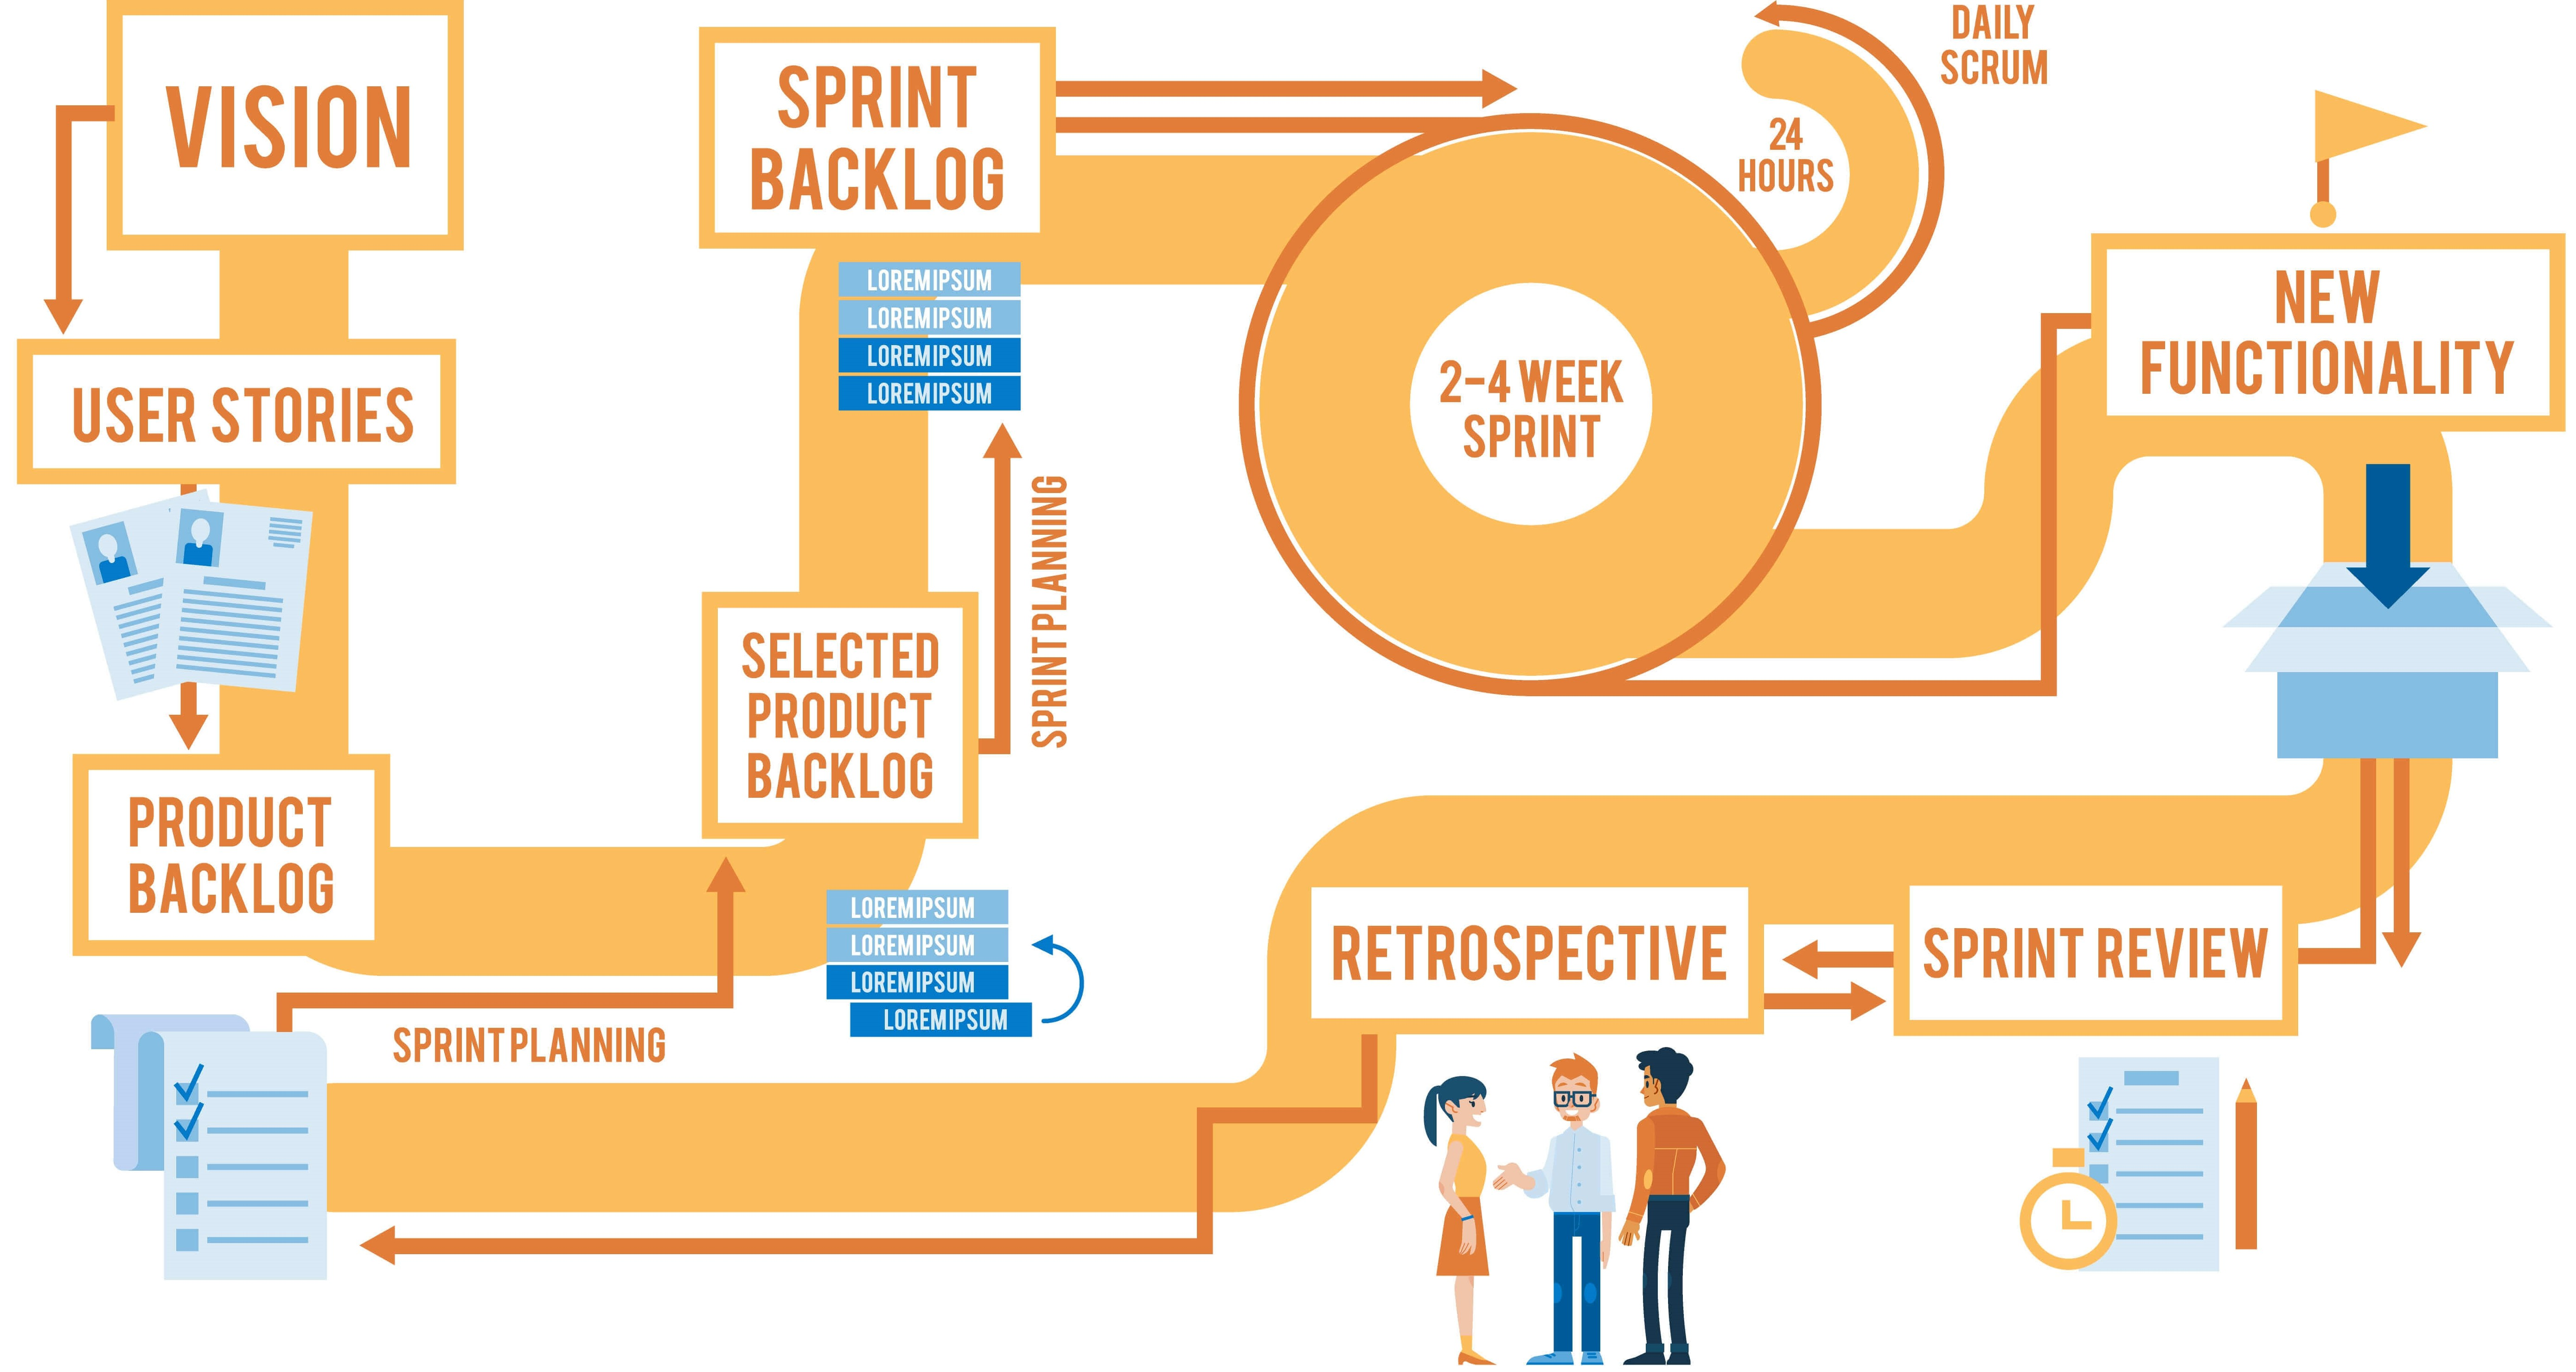
\includegraphics[scale = 0.08]{template/images/scrum.jpg}
    \caption{Il framework Scrum}
    \label{fig:2.1} % Etichetta per il riferimento
\end{figure}
\pagebreak

\section{Pianificazione}
Lo sviluppo del progetto è suddiviso nelle seguenti fasi:
    \begin{itemize}
        \item  RTB
        \item PB
    \end{itemize}
    \subsection{RTB}
    Nel periodo dal 04/11/2024 al 17/01/2025 verranno prodotti i seguenti documenti:
        \begin{itemize}
            \item "Norme di progetto"
            \item "Piano di progetto"
            \item "Analisi dei requisiti"
            \item "Piano di qualifica"
            \item "Glossario"
        \end{itemize}
    Inoltre verrà realizzato il Proof of Concept, per valutare la fattibilità tecnologica del progetto.
        \subsubsection{Sprint 1 (dal 11/11/2024 al 22/11/2024)}
        In questo periodo verrà definito il way of working, documentato nelle
        \textit{"Norme di progetto"}. Per quanto riguarda la gestione di progetto, verranno 
        pianificate le attività, stilato un preventivo e analizzati i rischi che potrebbero
        incidere sullo svolgimento del progetto. Infine si comincerà a redigere il 
        \textit{"Glossario"}, fondamentale per garantire una chiara comprensione e comunicazione all'
        interno del team e con il proponente.
        \\
        \begin{figure}[h!]
            \centering
            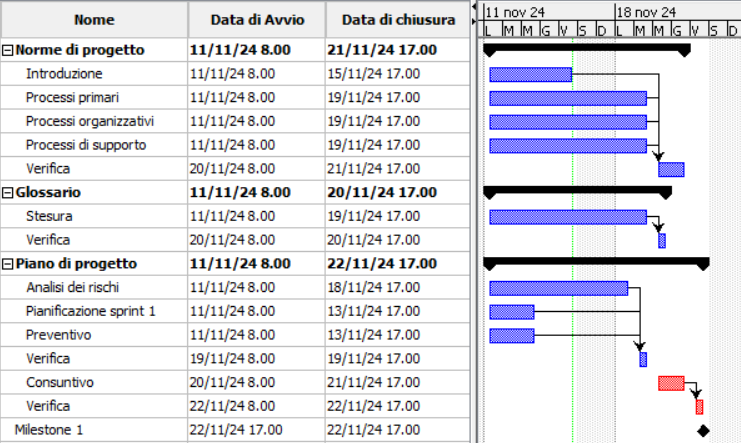
\includegraphics[scale = 0.85]{template/images/gantt1.png}
            \caption{Diagramma di Gantt sprint 1}
            \label{fig:3.1} % Etichetta per il riferimento
        \end{figure}

        \subsubsection{Sprint 2 (dal 25/11/2024 al 06/12/2024)}
     Durante questo secondo sprint, ci dedicheremo alla raccolta e all'analisi dei requisiti, identificando i casi d'uso. Questi saranno documentati nel file \textit{"Analisi dei requisiti"} per garantire una visione chiara degli obiettivi del progetto. Continueremo inoltre l'espansione del \textit{"glossario"}, già avviato durante lo sprint 1.  Procederemo con l'aggiornamento delle \textit{"Norme di Progetto"} tramite modifiche e miglioramenti per assicurare una gestione ottimale delle attività e delle risorse. infine, con priorità minore, inizieremo la stesura del \textit{"Piano di Qualifica"}, necessario per definire le metriche e le modalità di 
     verifica della qualità del prodotto.

        
        \begin{figure}[h!]
            \centering
            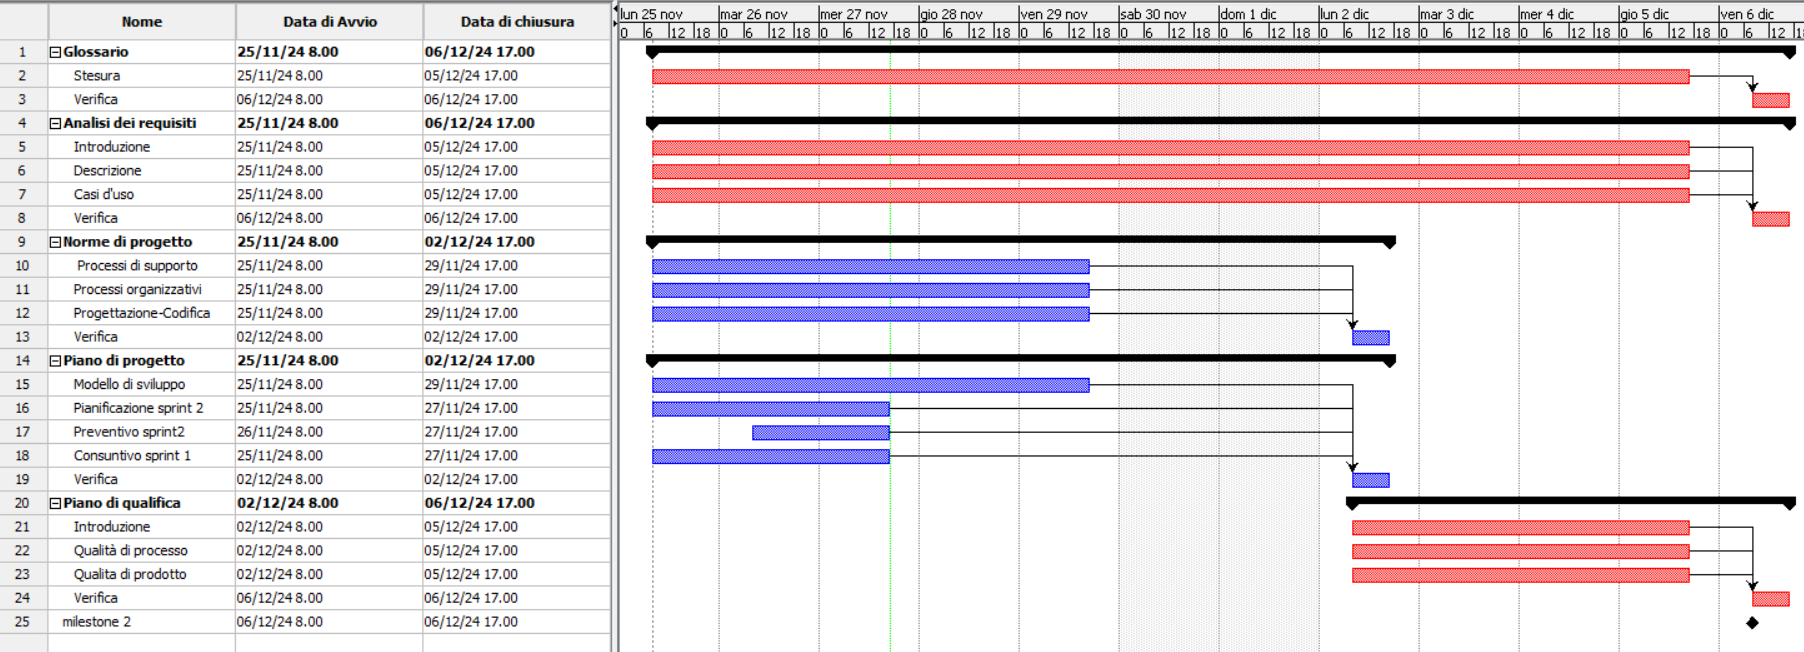
\includegraphics[scale = 0.3]{template/images/gantt2.png}
            \caption{Diagramma di Gantt sprint 2}
            \label{fig:3.1} % Etichetta per il riferimento
        \end{figure}
 

\pagebreak

\section{Preventivo}
In questa sezione viene pianificata nel dettaglio la suddivisione dei ruoli con
le corrispondenti ore di lavoro per ogni componente del gruppo e viene fornito
un preventivo, sia relativamente all'intera durata del progetto, sia
relativamente ad ogni periodo di lavoro.

\subsection{Ore totali}
Il team ha deciso di suddividere le ore individuali in modo equivalente,
assegnando un totale di 92 ore a ciascun membro. Di seguito si riporta la
distribuzione delle ore per ruolo e il calcolo dei costi totali.


\newcommand{\roleTable}[1]{

	\renewcommand{\arraystretch}{1.5}
	\rowcolors{2}{pari}{dispari}
	\begin{longtable}{ %0.87
		>{\centering}M{0.20\textwidth}
		>{\centering}M{0.10\textwidth}
		>{\centering}M{0.10\textwidth}
		>{\centering}M{0.10\textwidth}
		>{\centering\arraybackslash}M{0.15\textwidth}
		}
		\rowcolorhead
		\headertitle{Ruolo}           &
		\centering
		\headertitle{Ore ind.}        &
		\headertitle{Ore tot.}        &
		\headertitle{Costo (\euro/h)} &
		\headertitle{Costo Totale (\euro)}
		\endfirsthead
		\endhead

		#1

	\end{longtable}
	\vspace{1em}

}

    \roleTable{
    Responsabile& 9 & 54 & 30 &  1620\tabularnewline
    Amministratore& 7 & 42 & 20 &  840\tabularnewline
    Analista& 16 & 96 & 25 &  2400\tabularnewline
	Progettista& 20 & 120 & 25 &  3000\tabularnewline
	Programmatore & 22 & 132 & 15 &  1980 \\
    	Verificatore& 18 & 108 & 15 &  1620\tabularnewline
     \midrule[\heavyrulewidth] 
     \textbf{TOTALE}& 92 & 552 & - &  11460\tabularnewline

     \rowcolor{white}\caption{Distribuzione delle ore e costi totali}
    }





\subsection{Costo Totale}
Il costo finale calcolato in base alle tariffe orarie dei ruoli e alle ore
preventivate risulta di: \textbf{\euro 11460}.
\pagebreak
\subsection{RTB}
\subsubsection{Sprint 1}
Per il primo sprint, i ruoli necessari per raggiungere gli obiettivi
pianificati sono:
\begin{itemize}
    \item Responsabile;
    \item Amministratore;
    \item Verificatore;
    \item Analista.
\end{itemize}

Di seguito una tabella dettagliata con la distribuzione dei ruoli e delle ore previsti per ciascun membro.


\newcommand{\memberTable}[1]{

\renewcommand{\arraystretch}{1.5}
\rowcolors{2}{pari}{dispari}
\begin{longtable}{ %0.87
		>{\centering}M{0.22\textwidth} 
		>{\centering}M{0.08\textwidth}
		>{\centering}M{0.08\textwidth}
		>{\centering}M{0.08\textwidth} 
        >{\centering}M{0.08\textwidth} 
        >{\centering}M{0.08\textwidth} 
        >{\centering}M{0.08\textwidth} 
		>{\centering\arraybackslash}M{0.08\textwidth} 
		 }
	\rowcolorhead
	\headertitle{Membro} &	
    \headertitle{Resp.} &
	\headertitle{Amm.} &
	\headertitle{An.} & 
	\headertitle{Proge.} &
    \headertitle{Progr.} &
    \headertitle{Ver.} &
    \headertitle{TOT.}
	\endfirsthead	
	\endhead
	
	#1

\end{longtable}
\vspace{1em}

}

\memberTable{
    Bergamin Elia & 5 & - & - & - & - & - & \textbf{5}\tabularnewline
    Diviesti Filippo & - & - & - & - & - & 6 & \textbf{6}\tabularnewline
    Djossa Edgar & - & 5 & - & - & - & - & \textbf{5}\tabularnewline
    Chilese Elena & - & - & 7 & - & - & - & \textbf{7}\tabularnewline
    Pincin Matteo & - & - & - & - & - & 6 & \textbf{6}\tabularnewline
    Soranzo Andrea & - & 5 & - & - & - & - & \textbf{5}\tabularnewline
    \midrule[\heavyrulewidth]
    \textbf{TOTALE}& 5 & 10 & 7 & - & - & 12 &  34\tabularnewline

    \rowcolor{white}\caption{ Distribuzione delle ore preventivate per lo sprint 1}

}


I costi stimati per il primo sprint sono riportati nella tabella seguente:


\newcommand{\costTable}[1]{

\renewcommand{\arraystretch}{1.5}
\rowcolors{2}{pari}{dispari}
\begin{longtable}{ %0.87
		>{\centering}M{0.20\textwidth} 
		>{\centering}M{0.10\textwidth}
		>{\centering}M{0.10\textwidth}
		>{\centering}M{0.10\textwidth} 
		>{\centering\arraybackslash}M{0.15\textwidth} 
		 }
	\rowcolorhead
	\headertitle{Ruolo} &
	\centering 
    \headertitle{Ore} &	
	\headertitle{Costo  (\euro/h)} &
    \headertitle{Costo Totale (\euro)}
	\endfirsthead	
	\endhead
	
	#1

\end{longtable}
\vspace{1em}

}

\costTable{
    Responsabile & 5 & 30 & 150 \tabularnewline
    Amministratore & 10 & 20 & 200 \tabularnewline
    Analista & 7 & 25 & 175 \tabularnewline
    Progettista & - & 25 & - \tabularnewline
    Programmatore & - & 15 & - \tabularnewline
    Verificatore & 12 & 15 & 180 \tabularnewline
    \midrule[\heavyrulewidth]
    \textbf{TOTALE} & 34 & - & 705 \tabularnewline

    \rowcolor{white}\caption{Preventivo costi sprint 1}

}


\pagebreak 
\subsubsection{Sprint 2}
Per il secondo sprint, i ruoli necessari per raggiungere gli obiettivi
pianificati sono:
\begin{itemize}
    \item Responsabile;
    \item Amministratore;
    \item Verificatore;
    \item Analista.
\end{itemize}


Di seguito una tabella dettagliata con la distribuzione dei ruoli e delle ore previsti per ciascun membro.


\memberTable{
    Bergamin Elia & - & - & - & - & - & 7 & \textbf{7}\tabularnewline
    Diviesti Filippo & - & - & 9 & - & - & - & \textbf{9}\tabularnewline
    Djossa Edgar & 5 & - & - & - & - & - & \textbf{5}\tabularnewline
    Chilese Elena & - & 7 & - & - & - & - & \textbf{7}\tabularnewline
    Pincin Matteo & - & - & 9 & - & - & - & \textbf{9}\tabularnewline
    Soranzo Andrea & - & - & - & - & - & 7 & \textbf{7}\tabularnewline
    \midrule[\heavyrulewidth]
    \textbf{TOTALE}& 5 & 7 & 18 & - & - & 14 &  44\tabularnewline

    \rowcolor{white}\caption{ Distribuzione delle ore preventivate per lo sprint 2}

}


I costi stimati per il secondo sprint sono riportati nella tabella seguente:


\costTable{
    Responsabile & 5 & 30 & 150 \tabularnewline
    Amministratore & 7 & 20 & 140 \tabularnewline
    Analista & 18 & 25 & 450 \tabularnewline
    Progettista & - & 25 & - \tabularnewline
    Programmatore & - & 15 & - \tabularnewline
    Verificatore & 14 & 15 & 210 \tabularnewline
    \midrule[\heavyrulewidth]
    \textbf{TOTALE} & 44 & - & 950 \tabularnewline

    \rowcolor{white}\caption{ Preventivo costi sprint 2}

}


\pagebreak 
\subsubsection{Sprint 3}
Per il terzo sprint, i ruoli necessari per raggiungere gli obiettivi
pianificati sono:
\begin{itemize}
    \item Responsabile;
    \item Amministratore;
    \item Verificatore;
    \item Analista.
\end{itemize}


Di seguito una tabella dettagliata con la distribuzione dei ruoli e delle ore previste per ciascun membro.


\memberTable{
    Bergamin Elia & - & 1 & 8 & - & - & - & \textbf{9}\tabularnewline
    Diviesti Filippo & 3 & - & - & - & - & - & \textbf{3}\tabularnewline
    Djossa Edgar & - & - & - & - & - & 3 & \textbf{3}\tabularnewline
    Chilese Elena & - & - & - & - & - & 3 & \textbf{3}\tabularnewline
    Pincin Matteo & - & 2 & - & - & - & - & \textbf{2}\tabularnewline
    Soranzo Andrea & - & - & 7 & - & - & - & \textbf{7}\tabularnewline
    \midrule[\heavyrulewidth]
    \textbf{TOTALE}& 3 & 3 & 15 & - & - & 6 & \textbf{27}\tabularnewline

    \rowcolor{white}\caption{Distribuzione delle ore preventivate per lo sprint 3}

}


I costi stimati per il terzo sprint sono riportati nella tabella seguente:


\costTable{
    Responsabile & 3 & 30 & 90 \tabularnewline
    Amministratore & 3 & 20 & 60 \tabularnewline
    Analista & 15 & 25 & 375 \tabularnewline
    Progettista & - & 25 & - \tabularnewline
    Programmatore & - & 15 & - \tabularnewline
    Verificatore & 6 & 15 & 90 \tabularnewline
    \midrule[\heavyrulewidth]
    \textbf{TOTALE} & 27 & - & 615 \tabularnewline

    \rowcolor{white}\caption{Preventivo costi sprint 3}

}


\pagebreak 
\subsubsection{Sprint 4}
Per il quarto sprint, i ruoli necessari per raggiungere gli obiettivi
pianificati sono:
\begin{itemize}
    \item Responsabile;
    \item Amministratore;
    \item Analista;
    \item Programmatore;
    \item Verificatore.
\end{itemize}


Di seguito una tabella dettagliata con la distribuzione dei ruoli e delle ore previste per ciascun membro.


\memberTable{
    Bergamin Elia & - & - & - & - & 3 & 2.5 & \textbf{5.5}\tabularnewline
    Diviesti Filippo & - & 2 & - & - & - & - & \textbf{2}\tabularnewline
    Djossa Edgar & - & - & 2 & - & - & - & \textbf{2}\tabularnewline
    Chilese Elena & 3 & - & - & - & - & - & \textbf{3}\tabularnewline
    Pincin Matteo & - & - & - & - & 3 & - & \textbf{3}\tabularnewline
    Soranzo Andrea & - & 2 & - & - & - & 5 & \textbf{8}\tabularnewline
    \midrule[\heavyrulewidth]
    \textbf{TOTALE}& 3 & 4 & 2 & - & 6 & 7.5 & \textbf{22.5} \tabularnewline

    \rowcolor{white}\caption{Distribuzione delle ore preventivate per lo sprint 4}

}


I costi stimati per il quarto sprint sono riportati nella tabella seguente:


\costTable{
    Responsabile & 3 & 30 & 90 \tabularnewline
    Amministratore & 4 & 20 & 80 \tabularnewline
    Analista & 2 & 25 & 50 \tabularnewline
    Progettista & - & 25 & - \tabularnewline
    Programmatore & 6 & 15 & 90 \tabularnewline
    Verificatore & 7.5 & 15 & 112.5 \tabularnewline
    \midrule[\heavyrulewidth]
    \textbf{TOTALE} & 22.5 & - & 422.5 \tabularnewline

    \rowcolor{white}\caption{ Preventivo costi sprint 4}

}


\pagebreak
\subsubsection{Sprint 5}
Per il quinto sprint, i ruoli necessari per raggiungere gli obiettivi
pianificati sono:
\begin{itemize}
    \item Responsabile;
    \item Amministratore;
    \item Analista;
    \item Programmatore;
    \item Verificatore.
\end{itemize}


Di seguito una tabella dettagliata con la distribuzione dei ruoli e delle ore previste per ciascun membro.


\memberTable{
    Bergamin Elia & - & 2 & - & - & - & 3 & \textbf{5}\tabularnewline
    Diviesti Filippo & - & - & - & - & - & 4 & \textbf{4}\tabularnewline
    Djossa Edgar & - & - & 2 & - & 2 & - & \textbf{4}\tabularnewline
    Chilese Elena & - & - & 2 & - & - & 3 & \textbf{5}\tabularnewline
    Pincin Matteo & 6 & - & - & - & - & - & \textbf{6}\tabularnewline
    Soranzo Andrea & - & - & 6 & - & - & - & \textbf{6}\tabularnewline
    \midrule[\heavyrulewidth]
    \textbf{TOTALE}& 6 & 2 & 10 & - & 2 & 10 & 30 \tabularnewline

    \rowcolor{white}\caption{ Distribuzione delle ore preventivate per lo sprint 5}

}


I costi stimati per il quinto sprint sono riportati nella tabella seguente:


\costTable{
    Responsabile & 6 & 30 & 180 \tabularnewline
    Amministratore & 2 & 20 & 40 \tabularnewline
    Analista & 10 & 25 & 250 \tabularnewline
    Progettista & - & 25 & - \tabularnewline
    Programmatore & 2 & 15 & 30 \tabularnewline
    Verificatore & 10 & 15 & 150 \tabularnewline
    \midrule[\heavyrulewidth]
    \textbf{TOTALE} & 30 & - & 650 \tabularnewline

    \rowcolor{white}\caption{Preventivo costi sprint 5}

}


\pagebreak 
\subsubsection{Sprint 6}
Per il sesto sprint, i ruoli necessari per raggiungere gli obiettivi
pianificati sono:
\begin{itemize}
    \item Responsabile;
    \item Amministratore;
    \item Analista;
    \item Verificatore.
\end{itemize}


Di seguito una tabella dettagliata con la distribuzione dei ruoli e delle ore previste per ciascun membro.


\memberTable{
    Bergamin Elia & - & - & - & - & - & 2 & \textbf{2}\tabularnewline
    Diviesti Filippo & - & 1 & - & - & - & - & \textbf{1}\tabularnewline
    Djossa Edgar & - & - & 1 & - & - & - & \textbf{1}\tabularnewline
    Chilese Elena & - & - & 2 & - & - & - & \textbf{2}\tabularnewline
    Pincin Matteo & - & - & - & - & - & 2 & \textbf{2}\tabularnewline
    Soranzo Andrea & 2 & - & - & - & - & - & \textbf{2}\tabularnewline
    \midrule[\heavyrulewidth]
    \textbf{TOTALE}& 2 & 1 & 3 & - & - & 4 & \textbf{10} \tabularnewline

    \rowcolor{white}\caption{Distribuzione delle ore preventivate per lo sprint 6}

}


I costi stimati per il sesto sprint sono riportati nella tabella seguente:


\costTable{
    Responsabile & 2 & 30 & 60 \tabularnewline
    Amministratore & 1 & 20 & 20 \tabularnewline
    Analista & 3 & 25 & 75 \tabularnewline
    Progettista & - & 25 & - \tabularnewline
    Programmatore & - & 15 & - \tabularnewline
    Verificatore & 4 & 15 & 60 \tabularnewline
    \midrule[\heavyrulewidth]
    \textbf{TOTALE} & 10 & - & 215 \tabularnewline

    \rowcolor{white}\caption{Preventivo costi sprint 6}

}

\pagebreak 
\subsubsection{Sprint 7}

Per il settimo sprint, i ruoli necessari per raggiungere gli obiettivi
pianificati sono:
\begin{itemize}
    \item Responsabile;
    \item Amministratore;
    \item Analista;
    \item Programmatore;
    \item Verificatore.
\end{itemize}


Di seguito una tabella dettagliata con la distribuzione dei ruoli e delle ore previste per ciascun membro.


\memberTable{
    Bergamin Elia & 2 & - & - & - & - & - & \textbf{2}\tabularnewline
    Diviesti Filippo & - & - & - & - & - & 1 & \textbf{1}\tabularnewline
    Djossa Edgar & - & 2 & - & - & - & - & \textbf{2}\tabularnewline
    Chilese Elena & - & 1 & - & - & - & 1 & \textbf{2}\tabularnewline
    Pincin Matteo & - & - & 3 & - & - & - & \textbf{3}\tabularnewline
    Soranzo Andrea & - & - & - & - & 2 & - & \textbf{2}\tabularnewline
    \midrule[\heavyrulewidth]
    \textbf{TOTALE}& 2 & 3 & 3 & - & 2 & 2 & \textbf{12} \tabularnewline

    \rowcolor{white}\caption{Distribuzione delle ore preventivate per lo sprint 7}

}


I costi stimati per il settimo sprint sono riportati nella tabella seguente:


\costTable{
    Responsabile & 2 & 30 & 60 \tabularnewline
    Amministratore & 3 & 20 & 60 \tabularnewline
    Analista & 3 & 25 & 75 \tabularnewline
    Progettista & - & 25 & - \tabularnewline
    Programmatore & 2 & 15 & 30 \tabularnewline
    Verificatore & 2 & 15 & 30 \tabularnewline
    \midrule[\heavyrulewidth]
    \textbf{TOTALE} & 12 & - & 255 \tabularnewline

    \rowcolor{white}\caption{Preventivo costi sprint 7}

}


\pagebreak 
\subsubsection{Sprint 8}

Per l'ottavo sprint, i ruoli necessari per raggiungere gli obiettivi
pianificati sono:
\begin{itemize}
    \item Responsabile;
    \item Amministratore;
    \item Analista;
    \item Verificatore.
\end{itemize}


Di seguito una tabella dettagliata con la distribuzione dei ruoli e delle ore previste per ciascun membro.


\memberTable{
    Bergamin Elia & - & - & - & - & - & 1 & \textbf{1}\tabularnewline
    Diviesti Filippo & - & 1 & - & - & - & - & \textbf{1}\tabularnewline
    Djossa Edgar & - & - & - & - & - & 1 & \textbf{1}\tabularnewline
    Chilese Elena & - & - & 3 & - & - & - & \textbf{3}\tabularnewline
    Pincin Matteo & - & 1 & - & - & - & - & \textbf{1}\tabularnewline
    Soranzo Andrea & 3.5 & - & - & - & - & - & \textbf{3.5}\tabularnewline
    \midrule[\heavyrulewidth]
    \textbf{TOTALE}& 3.5 & 2 & 3 & - & - & 2 & \textbf{10.5} \tabularnewline

    \rowcolor{white}\caption{Distribuzione delle ore preventivate per lo sprint 8}

}


I costi stimati per il settimo sprint sono riportati nella tabella seguente:


\costTable{
    Responsabile & 3.5 & 30 & 105 \tabularnewline
    Amministratore & 2 & 20 & 40 \tabularnewline
    Analista & 3 & 25 & 75 \tabularnewline
    Progettista & - & 25 & - \tabularnewline
    Programmatore & - & 15 & - \tabularnewline
    Verificatore & 2 & 15 & 30 \tabularnewline
    \midrule[\heavyrulewidth]
    \textbf{TOTALE} & 10.5 & - & 250 \tabularnewline

    \rowcolor{white}\caption{Preventivo costi sprint 8}

}

\pagebreak

\section{Consuntivo}
\subsection{Introduzione}
Questa sezione riporta i dati raccolti durante il progetto riguardo alla ripartizione dei ruoli e alle ore impiegate da ogni componente del gruppo. Tali dati sono comparati alle previsioni presenti nella sezione di preventivo.

\subsection{Dettaglio Sprint}

\subsubsection{Sprint 1}
Di seguito la suddivisione dei ruoli e le ore di lavoro effettive impiegate in questo sprint:


\newcommand{\memberReportTable}[1]{

	\renewcommand{\arraystretch}{1.5}
	\rowcolors{2}{pari}{dispari}
	\begin{longtable}{ %0.87
		>{\centering}M{0.22\textwidth}
		>{\centering}M{0.08\textwidth}
		>{\centering}M{0.08\textwidth}
		>{\centering}M{0.08\textwidth}
		>{\centering}M{0.08\textwidth}
		>{\centering}M{0.08\textwidth}
		>{\centering}M{0.08\textwidth}
		>{\centering\arraybackslash}M{0.08\textwidth}
		}
		\rowcolorhead
		\headertitle{Membro} &
		\headertitle{Resp.}  &
		\headertitle{Amm.}   &
		\headertitle{An.}    &
		\headertitle{Proge.} &
		\headertitle{Progr.} &
		\headertitle{Ver.}   &
		\headertitle{TOT.}
		\endfirsthead
		\endhead

		#1

	\end{longtable}
	\vspace{1em}

}

\memberReportTable{
    Bergamin Elia       & 5 & - & - & - & - & - & \textbf{5}\tabularnewline
    Diviesti Filippo    & - & - & - & - & - & 6 & \textbf{6}\tabularnewline
    Djossa Edgar        & - & 5 & - & - & - & - & \textbf{5}\tabularnewline
    Chilese Elena       & - & - & 3 (-4) & - & - & - & \textbf{3 (-4)}\tabularnewline
    Pincin Matteo       & - & - & - & - & - & 6 & \textbf{6}\tabularnewline
    Soranzo Andrea      & - & 5 & - & - & - & - & \textbf{5}\tabularnewline
    \midrule[\heavyrulewidth]
    \textbf{TOTALE}     & 5 & 10 & 3 (-4) & - & - & 12 & \textbf{30 (-4)}\tabularnewline

    \rowcolor{white}\caption{Rendiconto effettivo della distribuzione delle ore per lo sprint 1}

}


I costi effettivi del periodo sono i seguenti:


\newcommand{\costReportTable}[1]{

	\renewcommand{\arraystretch}{1.5}
	\rowcolors{2}{pari}{dispari}
	\begin{longtable}{ %0.87
		>{\centering}M{0.30\textwidth}
		>{\centering}M{0.10\textwidth}
		>{\centering}M{0.10\textwidth}
		>{\centering}M{0.10\textwidth}
		>{\centering\arraybackslash}M{0.15\textwidth}
		}
		\rowcolorhead
		\headertitle{Ruolo}            &
		\centering
		\headertitle{Ore}              &
		\headertitle{Costo  (\euro/h)} &
		\headertitle{Costo Totale (\euro)}
		\endfirsthead
		\endhead

		#1

	\end{longtable}
	\vspace{1em}

}

\costReportTable{
    Responsabile & 5 & 30 & 150 \tabularnewline
    Amministratore & 10 & 20 & 200 \tabularnewline
    Analista & 3 (-4) & 25 & 75 (-100) \tabularnewline
    Progettista & - & 25 & - \tabularnewline
    Programmatore & - & 15 & - \tabularnewline
    Verificatore & 12 & 15 & 180 \tabularnewline
    \midrule[\heavyrulewidth]
    \textbf{Totale Consuntivo} & 30 & - & 605 \tabularnewline
    \midrule[\heavyrulewidth]
    \textbf{Totale Preventivo} & 34 & - & 705 \tabularnewline
    \midrule[\heavyrulewidth]
    \textbf{Differenza} & -4 & - & -100 \tabularnewline

    \rowcolor{white}\caption{Consuntivo costi sprint 1}

}


\subsubsubsection{Resoconto}
Nel seguente resoconto vengono analizzate le principali differenze tra le stime iniziali e le ore effettive durante lo sprint:
\begin{itemize}
    \item \textbf{Analista (-4 ore):} Alla fine sono state necessarie meno ore di lavoro da parte 
    dell'Analista rispetto al previsto. Questa variazione è legata, oltre che alla nostra inesperienza nel calcolo 
    accurato dei tempi necessari, principalmente ad impegni di altre materie universitarie.

\end{itemize}
Nel complesso, il lavoro svolto durante lo sprint è stato in linea con gli obiettivi prefissati, sebbene siano emerse alcune differenze rispetto alle stime iniziali.
\\
Per gli sprint successivi, sarà necessario affinare la fase di preventivazione, valutando con 
maggiore precisione la complessità delle attività, così da ottenere stime ancora più accurate.

\subsubsection{Sprint 2}
Di seguito la suddivisione dei ruoli e le ore di lavoro effettive impiegate in questo sprint:


\memberReportTable{
    Bergamin Elia & - & - & - & - & - & 7 & \textbf{7}\tabularnewline
    Diviesti Filippo & - & - & 9 & - & - & - & \textbf{9}\tabularnewline
    Djossa Edgar & 5 & - & - & - & - & - & \textbf{5}\tabularnewline
    Chilese Elena & - & 7 & - & - & - & - & \textbf{7}\tabularnewline
    Pincin Matteo & - & - & 9 & - & - & - & \textbf{9}\tabularnewline
    Soranzo Andrea & - & - & - & - & - & 7 & \textbf{7}\tabularnewline
    \midrule[\heavyrulewidth]
    \textbf{TOTALE}& 5 & 7 & 18 & - & - & 14 &  44\tabularnewline

    \rowcolor{white}\caption{ Rendiconto effettivo della distribuzione delle ore per lo sprint 2}

}


I costi effettivi del periodo sono i seguenti:


\costReportTable{
    Responsabile & 7 & 30 & 210 \tabularnewline
    Amministratore & 14 & 20 & 280 \tabularnewline
    Analista & 18 & 25 & 450 \tabularnewline
    Progettista & - & 25 & - \tabularnewline
    Programmatore & - & 15 & - \tabularnewline
    Verificatore & 14 & 15 & 210 \tabularnewline
    \midrule[\heavyrulewidth]
    \textbf{Totale Consuntivo} & 53 & - & 1150 \tabularnewline
    \midrule[\heavyrulewidth]
    \textbf{Totale Preventivo} & 44 & - & 950 \tabularnewline
    \midrule[\heavyrulewidth]
    \textbf{Differenza} & 9 & - & 200 \tabularnewline

    \rowcolor{white}\caption{ Consuntivo costi sprint 2}

}


\subsubsubsection{Resoconto}
Nel seguente resoconto vengono analizzate le principali differenze tra le stime iniziali e le ore effettive durante lo sprint:
\begin{itemize}
    \item \textbf{Verificatore (-2 ore);} 
    \item \textbf{Responsabile (+2 ore);} 
    \item \textbf{Amministratore (+5 ore).}
\end{itemize}
Sono state eseguite meno ore da verificatore poichè l'ammontare è stato leggermente sovrastimato. Inoltre le ore aggiuntive di responsabile e amministratore si evincono dal fatto che si ha avuto più tempo da dedicare al progetto rispetto
a quello preventivato.
\\
Nel complesso, anche grazie al lavoro aggiuntivo svolto, sono stati rispettati tutti gli obiettivi prefissati per questo sprint.

\subsubsection{Sprint 3}
Di seguito la suddivisione dei ruoli e le ore di lavoro effettive impiegate in questo sprint:


\memberReportTable{
    Bergamin Elia & - & 1 & 5 (-3) & - & - & - & \textbf{6}\tabularnewline
    Diviesti Filippo & 4 (+1) & - & - & - & - & - & \textbf{4}\tabularnewline
    Djossa Edgar & - & 0.5 (+0.5) & - & - & - & 5 (+2) & \textbf{5.5}\tabularnewline
    Chilese Elena & - & - & - & - & - & 4 (+1) & \textbf{4}\tabularnewline
    Pincin Matteo & - & 4 (+2) & - & - & - & - & \textbf{4}\tabularnewline
    Soranzo Andrea & - & - & 6 (-1) & - & - & - & \textbf{6}\tabularnewline
    \midrule[\heavyrulewidth]
    \textbf{TOTALE}& 4 & 5.5 & 11 & - & - & 9 &  29.5 \tabularnewline

    \rowcolor{white}\caption{Rendiconto effettivo della distribuzione delle ore per lo sprint 3}

}


I costi effettivi del periodo sono i seguenti:


\costReportTable{
    Responsabile & 4 (+1) & 30 & 120 \tabularnewline
    Amministratore & 5.5 (+1.5) & 20 & 110 \tabularnewline
    Analista & 11 (-4) & 25 & 275 \tabularnewline
    Progettista & - & 25 & - \tabularnewline
    Programmatore & - & 15 & - \tabularnewline
    Verificatore & 9 (+3) & 15 & 135 \tabularnewline
    \midrule[\heavyrulewidth]
    \textbf{Totale Consuntivo} & 29.5 & - & 640 \tabularnewline
    \midrule[\heavyrulewidth]
    \textbf{Totale Preventivo} & 27 & - & 615 \tabularnewline
    \midrule[\heavyrulewidth]
    \textbf{Differenza} & 2.5 & - & 25 \tabularnewline

    \rowcolor{white}\caption{ Consuntivo costi sprint 3}

}


\subsubsubsection{Resoconto}
Nel seguente resoconto vengono analizzate le principali differenze tra le stime iniziali e le ore effettive durante lo sprint:
\begin{itemize}
    \item \textbf{Responsabile (+1 ora);} 
    \item \textbf{Amministratore (+1.5 ore);} 
    \item \textbf{Analista (-4 ore);}
    \item \textbf{Verificatore (+3 ore);}
\end{itemize}

Sono state dedicate più ore al ruolo di responsabile e di amministratore rispetto a quanto inizialmente previsto, a causa di una maggiore complessità nella gestione e organizzazione delle attività progettuali.
Le ore destinate al ruolo di analista sono state inferiori alle stime, in quanto alcune attività di analisi sono risultate meno onerose del previsto ed hanno altresì aiutato il confronto con il proponente e l'incontro con il prof. Cardin. 
Infine, il ruolo di verificatore ha richiesto un incremento di ore rispetto al pianificato, in virtù di un aumento della complessità e dell'estensione dei documenti da verificare.
\\
Complessivamente, le variazioni riscontrate non hanno compromesso il raggiungimento degli obiettivi prefissati, permettendo il completamento di tutte le attività previste.

\pagebreak

\newcommand{\riskMitigation}[1]{%
    \renewcommand{\arraystretch}{1.5}% Modifica l'altezza delle righe
    \rowcolors{2}{pari}{dispari}% Alterna i colori delle righe
    \begin{longtable}{%
        >{\centering\arraybackslash}m{0.22\textwidth}%
        >{\centering\arraybackslash}m{0.38\textwidth}%
        >{\centering\arraybackslash}m{0.38\textwidth}%
    }%
        \rowcolorhead
        \headertitle{Nome} &
        \headertitle{Descrizione} &
        \headertitle{Mitigazione} \\
        \endfirsthead
        \endhead

        #1 % Contenuto dinamico

    \end{longtable}
    \vspace{1em}
}

\section{Attualizzazione dei rischi}
In questa sezione sono riportati i rischi che si sono verificati nel corso del progetto e le relative misure di mitigazione attuate dal gruppo.

\riskMitigation{
    \textbf{Comprensione dei requisiti} & I requisiti non erano chiari basandosi sul capitolato. & Si sono svolte delle riunioni con il proponente, per discutere e chiarire dubbi. \\
    \textbf{Inesperienza Tecnologica} & Nella fase iniziale del progetto, e durante lo sviluppo del PoC sono sorti dubbi e difficoltà rispetto all'utilizzo di GitHub e delle tecnologie proposte dall'azienda. & Ogni membro del gruppo si è impegnato per ricavare del tempo personale da dedicare allo studio delle tecnologie da utilizzare, in modo da essere allineati e procedere con maggiore efficienza. \\
    \textbf{Disponibilità dei componenti} & A causa delle festività, la disponibilità dei componenti del gruppo si è ridotta durante quello sprint. & Nella pianificazione si è tenuto conto di questo fattore, inoltre, lo sprint è durato una settimana in più.\\
    \textbf{Discussioni interne} & Durante gli sprint è capitato di dover prendere delle decisioni o di avere dei dubbi, che andassero risolti prima del meeting interno di fine periodo. & È stato usato il canale di comunicazione asincrono Telegram per poter discutere e arrivare a una conclusione.
}
\pagebreak


% insert here other content (\include)


\end{document}


